
\PassOptionsToPackage{table}{xcolor}
\documentclass[letterpaper]{article} % DO NOT CHANGE THIS
\usepackage[submission]{aaai2026}  % DO NOT CHANGE THIS
\usepackage{times}  % DO NOT CHANGE THIS
\usepackage{helvet}  % DO NOT CHANGE THIS
\usepackage{courier}  % DO NOT CHANGE THIS
\usepackage[hyphens]{url}  % DO NOT CHANGE THIS
\usepackage{graphicx} % DO NOT CHANGE THIS
\urlstyle{rm} % DO NOT CHANGE THIS
\def\UrlFont{\rm}  % DO NOT CHANGE THIS
\usepackage{natbib}  % DO NOT CHANGE THIS AND DO NOT ADD ANY OPTIONS TO IT
\usepackage{caption} % DO NOT CHANGE THIS AND DO NOT ADD ANY OPTIONS TO IT
\frenchspacing  % DO NOT CHANGE THIS
\setlength{\pdfpagewidth}{8.5in} % DO NOT CHANGE THIS
\setlength{\pdfpageheight}{11in} % DO NOT CHANGE THIS
%
% These are recommended to typeset algorithms but not required. See the subsubsection on algorithms. Remove them if you don't have algorithms in your paper.
\usepackage{algorithm}
\usepackage{algorithmic}

% YipanWei Edited
\usepackage[table]{xcolor}
\usepackage{multirow}
\usepackage{arydshln}

\definecolor{DarkGreen}{RGB}{34,120,50}


\newcommand{\pub}[1]{{\color{gray}{\footnotesize{[{#1}]}}}}

\newcommand{\tworowbestreshl}[2]{%
\begin{tabular}{@{}c@{}}
{#1}  \\
{\small\color{DarkGreen}{$+$ \textbf{#2\%}}}
\end{tabular}%
}

%
% These are are recommended to typeset listings but not required. See the subsubsection on listing. Remove this block if you don't have listings in your paper.
\usepackage{newfloat}
\usepackage{listings}
\DeclareCaptionStyle{ruled}{labelfont=normalfont,labelsep=colon,strut=off} % DO NOT CHANGE THIS
\lstset{%
	basicstyle={\footnotesize\ttfamily},% footnotesize acceptable for monospace
	numbers=left,numberstyle=\footnotesize,xleftmargin=2em,% show line numbers, remove this entire line if you don't want the numbers.
	aboveskip=0pt,belowskip=0pt,%
	showstringspaces=false,tabsize=2,breaklines=true}
\floatstyle{ruled}
\newfloat{listing}{tb}{lst}{}
\floatname{listing}{Listing}
%
% Keep the \pdfinfo as shown here. There's no need
% for you to add the /Title and /Author tags.
\pdfinfo{
/TemplateVersion (2026.1)
}
\definecolor{LAMPYellow}{RGB}{255,220,112}
\definecolor{HeaderGray}{RGB}{235,235,235}
\definecolor{AvgBlue}{RGB}{226,241,255}
\definecolor{GainGreen}{RGB}{32,132,84}
\definecolor{DropRed}{RGB}{190,54,54}
\newcommand{\tblhead}[1]{\strut #1}
\newcommand{\lampcell}[1]{\begingroup\setlength{\fboxsep}{0pt}\colorbox{LAMPYellow}{\makebox[6.7em][c]{\rule[-1.12ex]{0pt}{4.45ex}\bfseries\boldmath #1}}\endgroup}
\newcommand{\avgcell}[1]{\begingroup\def\avgcontent{#1}\def\avgheader{Avg}\ifx\avgcontent\avgheader\bfseries #1\else\setlength{\fboxsep}{0pt}\colorbox{AvgBlue}{\makebox[3.55em][c]{\strut #1}}\fi\endgroup}
\newcommand{\metriclampcell}[1]{\begingroup\setlength{\fboxsep}{0pt}\colorbox{LAMPYellow}{\makebox[7.05em][c]{\rule[-0.96ex]{0pt}{3.95ex}\bfseries\boldmath #1}}\endgroup}
\newcommand{\lampband}{\noalign{\begingroup\color{LAMPYellow}\hrule height 3.35ex\endgroup\kern-3.35ex}}
\newcommand{\headband}{\noalign{\begingroup\color{HeaderGray}\hrule height 6.15ex\endgroup\kern-6.15ex}}
\newcommand{\gainup}[1]{\makebox[5.85em][l]{\textcolor{DropRed}{\(\uparrow\)#1}}}
\newcommand{\gaindown}[1]{\makebox[5.85em][l]{\textcolor{DropRed}{\(\downarrow\)#1}}}
\newcommand{\dropdown}[1]{\makebox[5.85em][l]{\textcolor{DropRed}{\(\downarrow\)#1}}}
\newcommand{\neutraldelta}[1]{\makebox[5.85em][l]{\textcolor{GainGreen}{#1}}}
\newcommand{\compactdrop}[1]{\textcolor{DropRed}{\(\downarrow\)#1}}
\newcommand{\compactgain}[1]{\textcolor{DropRed}{\(\uparrow\)#1}}
\newcommand{\compactneutral}[1]{\textcolor{GainGreen}{#1}}

% DISALLOWED PACKAGES
% \usepackage{authblk} -- This package is specifically forbidden
% \usepackage{balance} -- This package is specifically forbidden
% \usepackage{color (if used in text)
% \usepackage{CJK} -- This package is specifically forbidden
% \usepackage{float} -- This package is specifically forbidden
% \usepackage{flushend} -- This package is specifically forbidden
% \usepackage{fontenc} -- This package is specifically forbidden
% \usepackage{fullpage} -- This package is specifically forbidden
% \usepackage{geometry} -- This package is specifically forbidden
% \usepackage{grffile} -- This package is specifically forbidden
% \usepackage{hyperref} -- This package is specifically forbidden
% \usepackage{navigator} -- This package is specifically forbidden
% (or any other package that embeds links such as navigator or hyperref)
% \indentfirst} -- This package is specifically forbidden
% \layout} -- This package is specifically forbidden
% \multicol} -- This package is specifically forbidden
% \nameref} -- This package is specifically forbidden
% \usepackage{savetrees} -- This package is specifically forbidden
% \usepackage{setspace} -- This package is specifically forbidden
% \usepackage{stfloats} -- This package is specifically forbidden
% \usepackage{tabu} -- This package is specifically forbidden
% \usepackage{titlesec} -- This package is specifically forbidden
% \usepackage{tocbibind} -- This package is specifically forbidden
% \usepackage{ulem} -- This package is specifically forbidden
% \usepackage{wrapfig} -- This package is specifically forbidden
% DISALLOWED COMMANDS
% \nocopyright -- Your paper will not be published if you use this command
% \addtolength -- This command may not be used
% \balance -- This command may not be used
% \baselinestretch -- Your paper will not be published if you use this command
% \clearpage -- No page breaks of any kind may be used for the final version of your paper
% \columnsep -- This command may not be used
% \newpage -- No page breaks of any kind may be used for the final version of your paper
% \pagebreak -- No page breaks of any kind may be used for the final version of your paperr
% \pagestyle -- This command may not be used
% \tiny -- This is not an acceptable font size.
% \vspace{- -- No negative value may be used in proximity of a caption, figure, table, section, subsection, subsubsection, or reference
% \vskip{- -- No negative value may be used to alter spacing above or below a caption, figure, table, section, subsection, subsubsection, or reference

\setcounter{secnumdepth}{0} %May be changed to 1 or 2 if section numbers are desired.

% The file aaai2026.sty is the style file for AAAI Press
% proceedings, working notes, and technical reports.
%

% Title

% Your title must be in mixed case, not sentence case.
% That means all verbs (including short verbs like be, is, using,and go),
% nouns, adverbs, adjectives should be capitalized, including both words in hyphenated terms, while
% articles, conjunctions, and prepositions are lower case unless they
% directly follow a colon or long dash

\title{LAMP-Merge: Long-tail-Aware Medical Prototype Merging for One-shot Asynchronous Clinical Models}
\author{
    %Authors
    % All authors must be in the same font size and format.
    Written by AAAI Press Staff\textsuperscript{\rm 1}\thanks{With help from the AAAI Publications Committee.}\\
    AAAI Style Contributions by Pater Patel Schneider,
    Sunil Issar,\\
    J. Scott Penberthy,
    George Ferguson,
    Hans Guesgen,
    Francisco Cruz\equalcontrib,
    Marc Pujol-Gonzalez\equalcontrib
}
\affiliations{
    %Afiliations
    \textsuperscript{\rm 1}Association for the Advancement of Artificial Intelligence\\
    % If you have multiple authors and multiple affiliations
    % use superscripts in text and roman font to identify them.
    % For example,

    % Sunil Issar\textsuperscript{\rm 2},
    % J. Scott Penberthy\textsuperscript{\rm 3},
    % George Ferguson\textsuperscript{\rm 4},
    % Hans Guesgen\textsuperscript{\rm 5}
    % Note that the comma should be placed after the superscript

    1101 Pennsylvania Ave, NW Suite 300\\
    Washington, DC 20004 USA\\
    % email address must be in roman text type, not monospace or sans serif
    proceedings-questions@aaai.org
%
% See more examples next
}

%Example, Single Author, ->> remove \iffalse,\fi and place them surrounding AAAI title to use it
\iffalse
\title{My Publication Title --- Single Author}
\author {
    Author Name
}
\affiliations{
    Affiliation\\
    Affiliation Line 2\\
    name@example.com
}
\fi

\iffalse
%Example, Multiple Authors, ->> remove \iffalse,\fi and place them surrounding AAAI title to use it
\title{My Publication Title --- Multiple Authors}
\author {
    % Authors
    First Author Name\textsuperscript{\rm 1},
    Second Author Name\textsuperscript{\rm 2},
    Third Author Name\textsuperscript{\rm 1}
}
\affiliations {
    % Affiliations
    \textsuperscript{\rm 1}Affiliation 1\\
    \textsuperscript{\rm 2}Affiliation 2\\
    firstAuthor@affiliation1.com, secondAuthor@affilation2.com, thirdAuthor@affiliation1.com
}
\fi


% REMOVE THIS: bibentry
% This is only needed to show inline citations in the guidelines document. You should not need it and can safely delete it.
\usepackage{bibentry}
% END REMOVE bibentry

\begin{document}

\maketitle

\begin{abstract}
Model merging aims to integrate multiple independently trained local checkpoints into a unified global model, typically through general-purpose paradigms such as parameter interpolation, task-vector composition, or update-direction alignment. These methods implicitly assume that client models share relatively complete and comparable global discriminative structures. We argue that this assumption does not hold in medical settings, giving rise to two diagnostic-structure anomalies: (1)\textbf{ Aggregation-induced prediction collapse after merging}: When clients have incomplete diagnostic-class coverage, multiple locally effective models can be merged into a globally collapsed model whose predictive distribution concentrates on a small number of dominant classes. (2)\textbf{ Long-tailed medical prevalence cannot be ignored}. Majority classes in medical data often reflect genuine clinical prevalence rather than merely data noise. To address these challenges, we propose \textbf{LAMP-Merge}, which recasts medical model merging from global parameter interpolation as class-level diagnostic-evidence reconstruction. Through \textbf{diagnostic prototype reconstruction(DPR)} and \textbf{long-tail prevalence calibration(LPC)}, LAMP-Merge constructs a global diagnostic model without exposing raw medical images or requiring multi-round federated communication. Experiments on the Blood, Derma, Organ-C, Organ-S, and Ultrasound medical imaging datasets show that LAMP-Merge outperforms existing model-merging methods in most client-averaged settings while substantially mitigating prediction collapse.

% Index Terms:medical model merging, asynchronous fusion, predictive collapse, long-tail calibration, privacy-preserving learning
\end{abstract}


% Uncomment the following to link to your code, datasets, an extended version or similar.
% You must keep this block between (not within) the abstract and the main body of the paper.
% \begin{links}
%     \link{Code}{https://aaai.org/example/code}
%     \link{Datasets}{https://aaai.org/example/datasets}
%     \link{Extended version}{https://aaai.org/example/extended-version}
% \end{links}

\section{Introduction}

Federated learning~\cite{pmlr-v54-mcmahan17a,li2020fedprox,karimireddy2020scaffold,kairouz2021advances} and model merging~\cite{izmailov2018averaging,pmlr-v162-wortsman22a,ilharco2023editingmodelstaskarithmetic,yadav2023tiesmergingresolvinginterferencemerging} provide two important collaboration routes for privacy-sensitive multicenter medical intelligence. Federated learning enables hospitals to train collaboratively without sharing raw data~\cite{sheller2020federated,rieke2020future}, while model merging further reduces communication and optimization costs by integrating independently trained local models after training~\cite{ainsworth2023gitrebasinmergingmodels,stoica2024zipit,wu_parameter_2025}. These paradigms are particularly attractive for \textbf{medical imaging}, because a single hospital rarely covers the full disease spectrum, while privacy regulations and device heterogeneity make centralizing raw medical images difficult ~\cite{kaissis2020secure,bonawitz2019towards,abadi2016deep}.

Despite their success on natural images and general visual tasks~\cite{izmailov2018averaging,pmlr-v162-wortsman22a,ilharco2023editingmodelstaskarithmetic,entezari2022role,ainsworth2023gitrebasinmergingmodels}, transferring these paradigms to medical data remains challenging. A key reason is that general-purpose model merging implicitly assumes that different client checkpoints contain relatively complete and comparable \textbf{global discriminative structures}; local models are expected to align through parameter space, task-vector space, update signs, or curvature statistics~\cite{yadav2023tiesmergingresolvinginterferencemerging,yu2024languagemodelssupermario,wu_parameter_2025,jin2025datalessknowledgefusionmerging}. This assumption does not hold in medical scenarios. Medical centers differ not only in device domains but also in diagnostic-class availability: some centers may mainly cover common diseases or specific examination types, while having few rare-disease samples~\cite{9557808,10.1371/journal.pmed.1002683,li2021fedbn}. The resulting local models are not complete replicas of the global task, but \textbf{partial diagnostic experts} supported by locally observed diseases.

As illustrated in Fig.~\ref{fig:intro-collapse}, we summarize these challenges as two diagnostic-structure abnormalities in medical model merging:
\begin{itemize}
    \item \textbf{Diagnostic evidence fragmented across isolated medical clients.} Each client has reliable supervision only for observed classes; thus, a local model may be locally discriminative but still lack evidence for the full global diagnostic space~\cite{9557808,li2021fedbn}.
    \item \textbf{Long-tailed Medical Image Prevalence.} Medical image datasets naturally follow a long-tailed distribution: a few common diagnostic classes dominate the  samples, while rare classes are underrepresented~\cite{BUDA2018249,5597285}. Under this imbalanced class prior, a merged model collapsed to the majority class can still obtain high Accuracy despite lacking complete multi-class discrimination.
\end{itemize}

\begin{figure}[t]
    \centering
    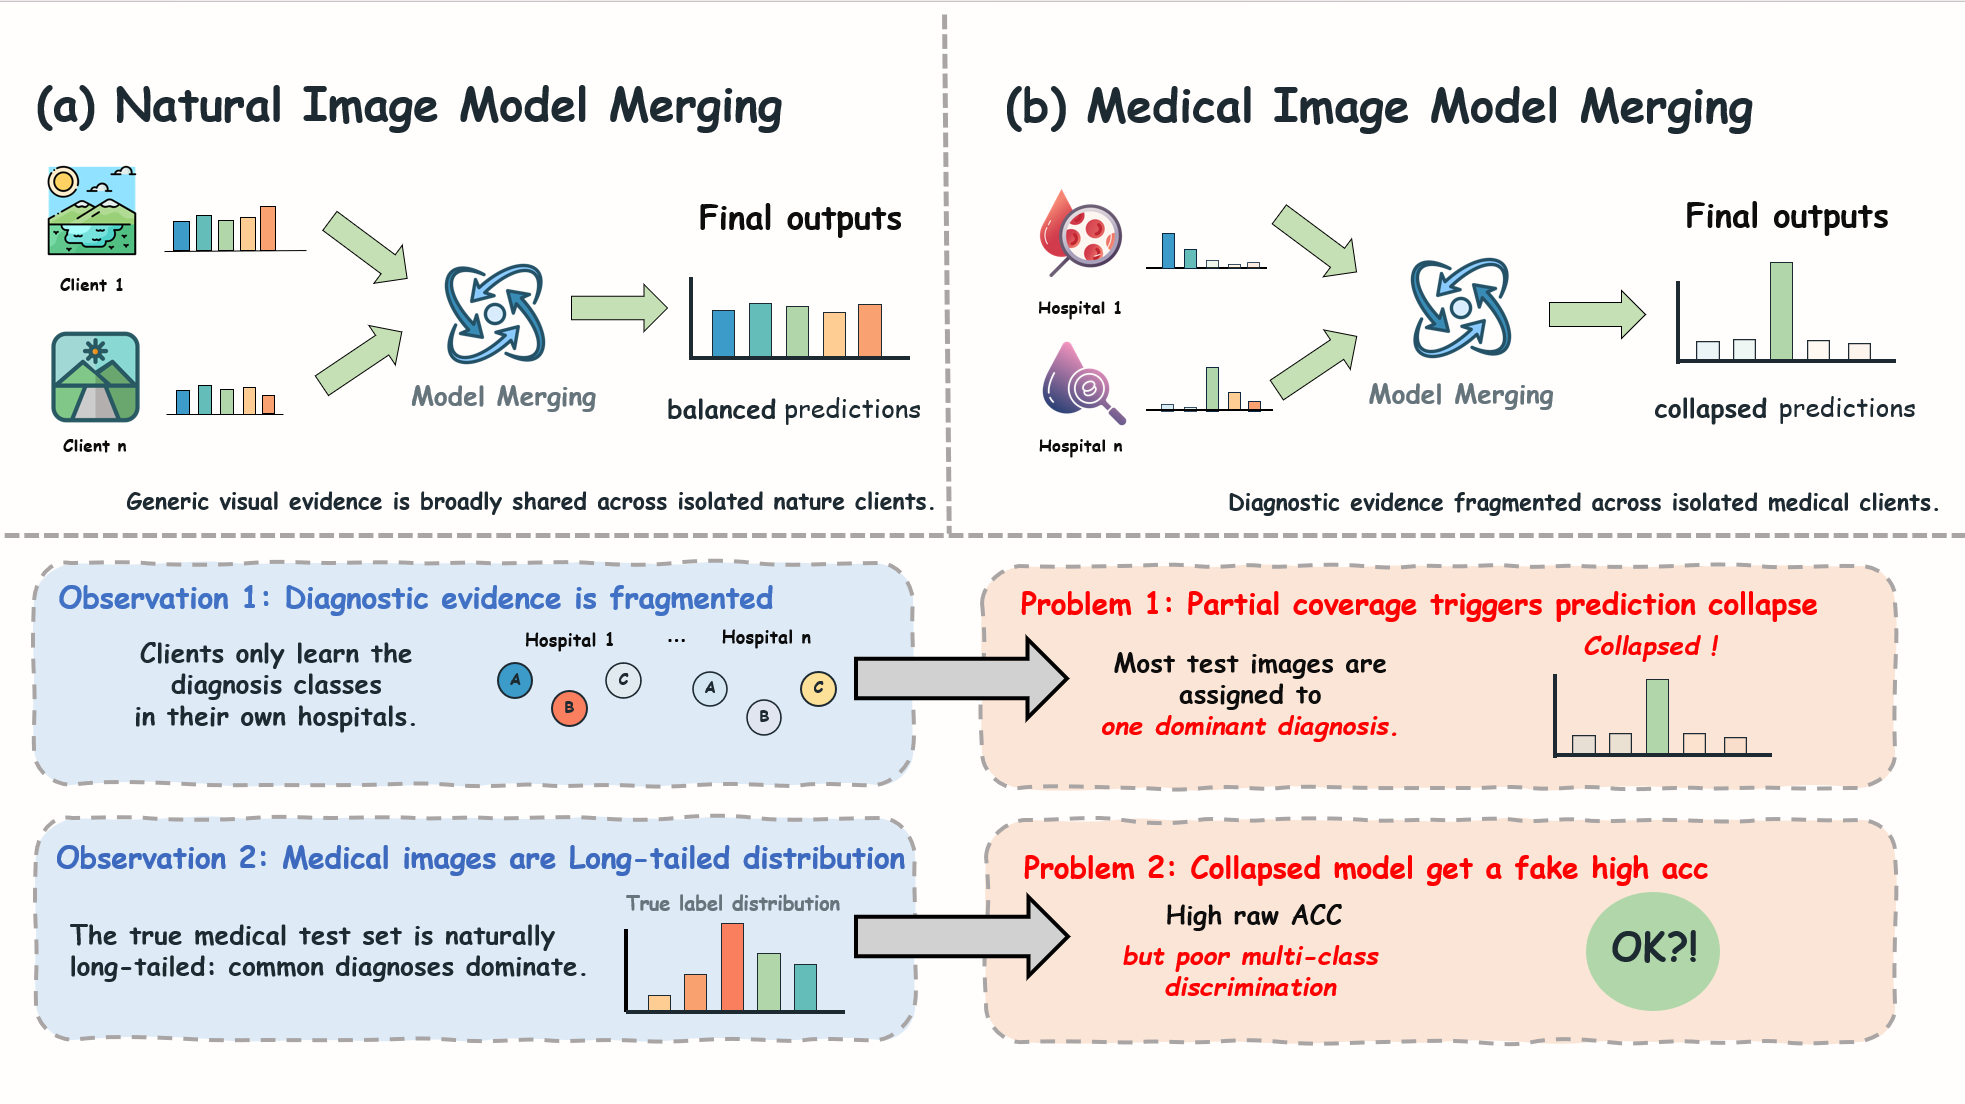
\includegraphics[width=0.96\linewidth]{figures/intro.png}
    \caption{In multicenter healthcare settings, individual clients typically observe only a subset of the global diagnostic space. Conventional parameter-level model-merging methods can therefore cause the merged global model's predictions to concentrate on a small number of dominant classes.}
    \label{fig:intro-collapse}
\end{figure}

To address these issues, we propose \textbf{LAMP-Merge, a long-tail-aware medical prototype-merging method for single-shot asynchronous medical image model merging}. LAMP-Merge shifts the merge target from global parameter interpolation to \textbf{class-level diagnostic-evidence reconstruction}. The key idea is to use client-uploaded class-level statistics as a synchronization signal for the global diagnostic space, allowing the server to reconstruct a global diagnostic classifier without accessing raw medical images, using a server-side validation set, or conducting multi-round federated communication. Specifically, LAMP-Merge consists of two mechanisms: \textbf{diagnostic prototype reconstruction} aggregates reliable class-level evidence through prototypes in a shared reference feature space, and \textbf{long-tail prevalence calibration} injects a bounded prior bias from client-uploaded class counts, thereby mitigating prediction collapse while preserving clinically meaningful majority-class prevalence.

\begin{figure*}[t]
    \centering
    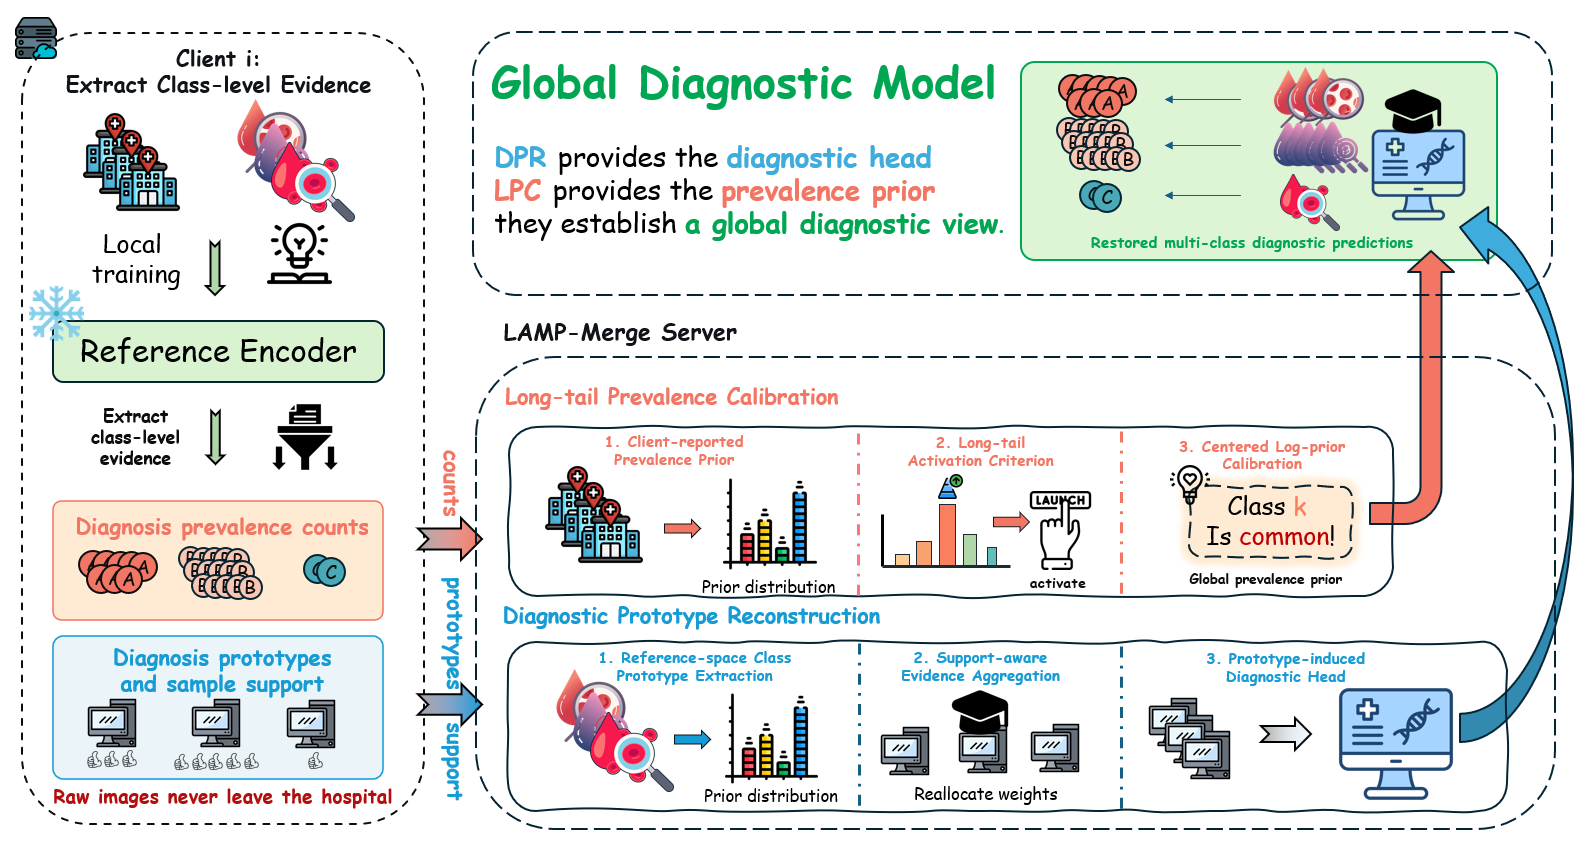
\includegraphics[width=0.92\textwidth,height=0.34\textheight]{figures/method.png}
    \caption{Local models from multicenter hospitals typically contain only partial diagnostic knowledge, while raw medical images cannot be centrally shared. LAMP-Merge reconstructs a privacy-friendly global medical classifier through DPR and LPC, without accessing raw data or requiring multi-round federated optimization.}
    \label{fig_method}
\end{figure*}

Our main contributions are summarized as follows:
\begin{itemize}
    \item \textbf{Medical Merging Diagnosis.} We revisit model merging under single-shot asynchronous medical collaboration and identify limited local diagnostic coverage and aggregation-induced prediction collapse as two key abnormalities caused by medical class availability and long-tailed prevalence.
    \item \textbf{LAMP-Merge.} We propose a long-tail-aware medical prototype-merging method that reconstructs a global diagnostic classifier from client-side class prototypes and prevalence statistics without exposing raw images or requiring multi-round federated optimization.
    \item \textbf{Empirical Validation.} We conduct full-scope experiments on five medical image datasets, four vision-model families, three client-population sizes, and three non-IID skew levels, showing that LAMP-Merge consistently outperforms strong model-merging baselines and improves prediction-collapse diagnostics.
\end{itemize}

\section{Related Works}

\subsection{Model Merging}

Model-merging methods integrate independently trained checkpoints in parameter, task-vector, or geometric spaces. Weight averaging~\cite{izmailov2018averaging} and Model Soups~\cite{pmlr-v162-wortsman22a} directly interpolate parameters; permutation-aware matching~\cite{entezari2022role,ainsworth2023gitrebasinmergingmodels} aligns hidden-unit symmetries; ZipIt~\cite{stoica2024zipit} performs feature-level zipping; Task Arithmetic~\cite{ilharco2023editingmodelstaskarithmetic}, TIES-Merging~\cite{yadav2023tiesmergingresolvinginterferencemerging}, and DARE~\cite{yu2024languagemodelssupermario} manipulate task deltas and sign conflicts; Fisher merging~\cite{wu_parameter_2025}, RegMean~\cite{jin2025datalessknowledgefusionmerging}, Model Stock~\cite{jang2025modelstockneedjust}, Breadcrumbs~\cite{davari2024modelbreadcrumbsscalingmultitask}, Iso-C~\cite{marczak2025taskleftbehindisotropic}, FreeMerge~\cite{zheng2025freemergingfouriertransformefficient}, and RobustMerge~\cite{zeng2025robustmergeparameterefficientmodelmerging} introduce curvature, mean-statistic, subspace, frequency-domain, or robustness assumptions.

However, these methods share a class-agnostic merging interface: their variables are global parameters, task vectors, update signs, or geometric statistics rather than class-level diagnostic evidence. \textbf{They do not encode whether a client has reliable supervision for a specific medical class.} Under incomplete local class coverage and long-tailed prevalence, reliable class directions can be mixed with absent or conflicting directions from other clients, resulting in aggregation-induced prediction collapse\cite{BUDA2018249,10.1371/journal.pmed.1002683}.

\subsection{Medical Model Merging}

Medical fusion studies exploit domain structures such as irregular clinical time series, physiological sensor graphs, and image-EHR fusion. mTAN~\cite{shukla2021multitimeattentionnetworksirregularly}, Raindrop~\cite{zhang2022graphguidednetworkirregularlysampled}, and MedFuse~\cite{hayat2023medfusemultimodalfusionclinical} show that medical tasks benefit from modeling clinical sampling mechanisms, modality heterogeneity, and patient-level temporal relations.

However, their fusion objects are usually patient-level inputs, multimodal records, or clinical representations rather than independently trained image-classifier checkpoints. They often require patient samples, timestamps, electronic health records, or server-side validation feedback, which conflicts with common privacy constraints~\cite{kaissis2020secure,sheller2020federated,bonawitz2019towards}. MedMerge~\cite{11382027} is a relevant training-free medical knowledge-transfer framework, but it targets cross-modal adaptation for medical vision-language models rather than asynchronous checkpoint merging for the same classification task. \textbf{Thus, existing medical fusion routes are mismatched with our privacy and single-upload protocol constraints.} LAMP-Merge keeps the medical structure uploadable by using only locally computed class prototypes and prevalence counts.

\subsection{Federated Learning}

Federated and decentralized learning perform collaborative training through communication protocols. FedAvg~\cite{pmlr-v54-mcmahan17a} and its variants or medical deployments~\cite{li2020fedprox,karimireddy2020scaffold,li2021fedbn,kaissis_secure_2020,sheller2020federated,rieke2020future,kairouz2021advances} rely on repeated server-client updates; Swarm Learning~\cite{warnat-herresthal_swarm_2021} and Gossip Learning~\cite{hegedhus_gossip_2019} reduce centralization but still require participants to continue training, exchanging models, and optimizing from intermediate states.

However, our setting begins after local training has finished. Hospitals may not remain online, receive global checkpoints repeatedly, or run additional optimization rounds. \textbf{The bottleneck is therefore communication feasibility in addition to privacy.} LAMP-Merge requires one upload of a local model interface and class-level statistics, enabling the server to construct a unified diagnostic model without a multi-round feedback loop.

\section{Method}

In this section, we first formulate the diagnostic-structure pathologies exposed when generic model merging is applied to medical data, namely \textbf{limited local diagnostic coverage} and \textbf{aggregation-induced prediction collapse}. To correct these intrinsic mismatches, we propose \textbf{LAMP-Merge}, a two-stage framework composed of \textbf{DPR} and \textbf{LPC}, as shown in Fig.~\ref{fig_method}.

\subsection{Preliminaries}

\subsubsection{Problem Formulation.}

Assume $K$ medical clients. Client $i$ owns a private labeled dataset $D_i=\{(x,y)\}$ drawn from a class-skewed medical distribution over $C$ diagnosis classes. Let $D_{i,c}$ denote the subset of client $i$ belonging to diagnosis class $c$. In medical partitions, $D_{i,c}$ can be empty for many classes; therefore, client $i$ has reliable supervision only for its observed classes. The goal is to construct a global diagnostic model under this partial and heterogeneous diagnostic-label coverage.

\subsubsection{Upload and Server Constraints.}

We study single-shot asynchronous merging: after local training, each client uploads only once, while the server cannot access raw medical images, per-sample features, per-sample predictions, or a server-side validation set, and does not issue multi-round updates to clients. Clients are allowed to upload class-level statistics. Specifically, $n_{i,c}$ denotes the class-support count, $m_{i,c}$ denotes the class-prevalence count, and $\mu_{i,c}$ denotes the class prototype computed in a shared reference feature space. The server performs one merge using only the local checkpoint interfaces and these class-level statistics. This setting differs from federated learning because clients do not continue optimization from server feedback; it also differs from standard model merging because the presence of class-level diagnostic evidence becomes an explicit merging variable.

\subsection{Motivation}

Although generic model merging is training-free and parameter-efficient, we find that its diagnostic structure can severely degenerate in medical model merging. Prediction-distribution diagnosis and class-support analysis reveal two key abnormalities:

\subsubsection{(1) Aggregation-induced prediction collapse.} Under partial diagnostic coverage, parameter-level merging can turn several locally useful predictors into \textbf{a globally collapsed predictor}. The merged model tends to allocate most test images to a few dominant classes, indicating that global class-discriminative structure has not been reconstructed.

\subsubsection{(2) Prevalence prior cannot be ignored.} Medical datasets often exhibit clinically meaningful long-tailed prevalence. Therefore, completely suppressing majority-class dominance is also inappropriate: a collapsed predictor is undesirable, but a merger should still preserve calibrated disease prevalence when the dominant class reflects the true clinical prior.

\subsection{Diagnostic Prototype Reconstruction Module}

To mitigate the \textbf{fragmented diagnostic evidence across isolated medical clients} caused by heterogeneous diagnostic coverage and conflicting class evidence, the diagnostic prototype reconstruction module shifts the merging target from parameter averaging to class-conditional evidence reconstruction. Instead of directly averaging local classifiers, it first collects reliable evidence for each diagnosis class in a shared reference space and then synthesizes a global diagnostic head over the full label space.

\subsubsection{(1) Reference-space Class Prototype Extraction.}


First, all clients extract class prototypes with the same frozen reference backbone. Let $\phi_0$ be the reference backbone instantiated from the shared model configuration before local training, and let $T(\cdot)$ be the evaluation transform. For each diagnosis class $c$, client $i$ locally computes a reference-space class prototype
\begin{equation}
\mu_{i,c}=\frac{1}{n_{i,c}}\sum_{(x,y)\in D_i}\mathbf{1}[y=c]\phi_0(T(x)),
\end{equation}
where $n_{i,c}=|D_{i,c}|$ is the class support count. If $n_{i,c}=0$, the client uploads zero support for that class and contributes no prototype evidence.

\subsubsection{(2) Support-aware Evidence Aggregation.}

Second, the server converts class-support counts into evidence weights to characterize the reliability of each client for a given class:
\begin{equation}
e_{i,c}=(n_{i,c}+1)^\gamma \mathbf{1}[n_{i,c}>0],
\end{equation}
where $\gamma=0.45$ is the default evidence exponent. This weight gives larger class-specific contribution to clients with more supervised samples of class $c$, while excluding clients that never observe this class. The normalized reliability is
\begin{equation}
\alpha_{i,c}=\frac{e_{i,c}}{\sum_{j=1}^{K} e_{j,c}}.
\end{equation}

The global diagnosis prototype is obtained by class-wise reliability-weighted aggregation:
\begin{equation}
p_c=\sum_{i=1}^{K}\alpha_{i,c}\mu_{i,c}.
\end{equation}
This step aggregates evidence only from clients that have actually observed class $c$, preventing absent-class classifiers from diluting valid diagnostic signals.

\subsubsection{(3) Prototype-induced Diagnostic Head.}

Finally, LAMP-Merge maps global diagnosis prototypes into a cosine prototype classifier:
\begin{equation}
w_c=s\frac{p_c}{\|p_c\|_2},
\end{equation}
where $s=20$ is the default head scale. The resulting head is not an average of local classifier parameters; it is induced by class evidence in the shared reference space, thereby restoring multiclass diagnostic directions over the global label space.

\subsection{Long-tail Prevalence Calibration}

To address the fact that \textbf{prevalence prior cannot be ignored} in real medical tasks, the long-tail prevalence calibration module introduces a bounded class prior after prototype reconstruction. This module does not push the model back to single-class collapse; instead, it calibrates the clinical prevalence reflected by client statistics after multiclass diagnostic directions have been restored.

\subsubsection{(1) Client-reported Prevalence Prior.}

First, each client uploads class-prevalence counts $m_{i,c}$. The server estimates the global class prior
\begin{equation}
\pi_c=\frac{\sum_{i=1}^{K}m_{i,c}}{\sum_{k=1}^{C}\sum_{i=1}^{K}m_{i,k}}.
\end{equation}
This prior is computed only from class-level counts, not from raw images, per-sample features, or per-sample predictions.

\subsubsection{(2) Long-tail Activation Criterion.}

Second, to avoid unnecessary calibration in non-long-tailed cases, the server measures dominant-class imbalance by
\begin{equation}
r=C\max_c \pi_c.
\end{equation}
The calibration module is activated only when $r>\tau$, where $\tau=2.5$ by default.

\subsubsection{(3) Centered Log-prior Calibration.}

Finally, when the module is activated, LAMP-Merge constructs a centered log-prior bias
\begin{equation}
b_c=\lambda\left(\log\pi_c-\frac{1}{C}\sum_{k=1}^{C}\log\pi_k\right),
\end{equation}
with default maximum calibration strength $\lambda=5.0$. The centering term prevents a uniform shift of all class logits, so the bias only changes the relative class prior. This module calibrates prevalence without replacing the diagnostic directions reconstructed by the first module.

\subsection{Optimization Objective and Algorithm}

The final scoring function of LAMP-Merge integrates the diagnostic prototype reconstruction term and the long-tail prevalence calibration term:
\begin{equation}
\ell_c(x)=w_c^\top\phi_0(T(x))+\mathbf{1}[r>\tau]\,b_c.
\end{equation}


\section{Experiments}

\subsection{Experimental Settings}

\subsubsection{(1) Evaluation Datasets:}

We evaluate the merged models on five representative MedMNIST v2 benchmarks\cite{yang2023medmnist}: Blood, Derma, Organ-C, Organ-S, and Ultrasound. They cover blood-cell microscopy, dermoscopy, abdominal CT, and ultrasound image classification (detailed dataset descriptions are provided in the Appendix).

\subsubsection{(2) Baselines:}

We compare LAMP-Merge with twelve model-merging baselines covering the main technical routes of current model merging: \texttt{avg}, \texttt{ties}\cite{yadav2023tiesmergingresolvinginterferencemerging}, \texttt{dare\_linear}\cite{yu2024languagemodelssupermario}, \texttt{dare\_ties}\cite{yu2024languagemodelssupermario}, \texttt{regmean}\cite{jin2025datalessknowledgefusionmerging}, \texttt{fisher}\cite{wu_parameter_2025}, \texttt{breadcrumbs}\cite{davari2024modelbreadcrumbsscalingmultitask}, \texttt{model\_stock}\cite{jang2025modelstockneedjust}, \texttt{from}\cite{ilharco2023editingmodelstaskarithmetic}, \texttt{iso\_c}\cite{marczak2025taskleftbehindisotropic}, \texttt{free\_merge}\cite{zheng2025freemergingfouriertransformefficient}, and \texttt{robustmerge}\cite{zeng2025robustmergeparameterefficientmodelmerging}. These baselines include weight averaging, task-vector pruning, sign-conflict resolution, curvature or mean-statistic correction, stock-style model interpolation, isotropic subspace merging, Fourier-domain fusion, and direction-robust merging.

\subsubsection{(3) Merging Settings:}

 
% Experiments follow a single-shot asynchronous model-merging protocol. Each client independently trains a local model on its own medical imaging data and then computes the class-level statistics required by LAMP-Merge locally, including class-support counts, reference-space class prototypes, and class-prevalence counts. These statistics are uploaded once together with an interface to the local checkpoint. The server performs a single model-merging step using only the uploaded checkpoints and class-level statistics, and evaluates the resulting merged model on a global test set.

We evaluate four vision-model families: ResNet, ConvNeXt, ViT-Tiny, and Swin-Tiny\cite{he2016deep,liu2022convnet,dosovitskiy2021image,liu2021swin}. For each dataset-model pair, we construct non-IID client partitions with $K\in\{3,5,7\}$ clients and Dirichlet skew parameter $\beta\in\{0,0.01,0.1\}$, using seed 42\cite{hsu2019measuringeffectsnonidenticaldata}. A client-average result fixes the dataset, model, and $K$, and then averages over the three $\beta$ values. And the experiments follow a single-shot asynchronous model-merging protocol.

% \subsubsection{4) Implementation Environment:}

% All experiments were run on a server with two Intel(R) Xeon(R) Silver 4210 CPUs, four NVIDIA GeForce RTX 2080 Ti GPUs, and the conda environment \texttt{MM} with Python 3.10.20, PyTorch 2.6.0+\texttt{cu118}, and CUDA runtime 11.8.

\subsection{Comparison With the State of the Arts}

% The main comparison uses client-average ACC: for each fixed dataset, model, and client number, we first average over the three $\beta$ skew levels and then compare merging methods. A cell is counted as successful when LAMP-Merge is greater than or equal to the strongest non-LAMP baseline in that cell.

Tables~\ref{tab:client-avg-resnet}--\ref{tab:client-avg-swin-tiny} report the full client-average results for all four backbones. Across the 60 client-average cells, LAMP-Merge wins or ties the strongest non-LAMP baseline in \textbf{57 cells (95.0\%)}.


% \begin{table*}[!p]
% \centering
% \scriptsize
% \setlength{\tabcolsep}{2.1pt}
% \caption{Client-average test accuracy (\%) on ResNet. Each entry averages the three Dirichlet settings for a fixed client number; Avg denotes the mean over $K=3,5,7$ within the corresponding dataset.}
% \label{tab:client-avg-resnet}
% \resizebox{\textwidth}{!}{%
% \begin{tabular}{lcccccccccccccccccccc}
% \hline
% \headband
% & \multicolumn{4}{c}{\tblhead{Blood}} & \multicolumn{4}{c}{\tblhead{Derma}} & \multicolumn{4}{c}{\tblhead{Organ-C}} & \multicolumn{4}{c}{\tblhead{Organ-S}} & \multicolumn{4}{c}{\tblhead{Ultrasound}} \\
% \cline{2-5}\cline{6-9}\cline{10-13}\cline{14-17}\cline{18-21}
% \tblhead{Method} & \tblhead{$K=3$} & \tblhead{$K=5$} & \tblhead{$K=7$} & \avgcell{Avg} & \tblhead{$K=3$} & \tblhead{$K=5$} & \tblhead{$K=7$} & \avgcell{Avg} & \tblhead{$K=3$} & \tblhead{$K=5$} & \tblhead{$K=7$} & \avgcell{Avg} & \tblhead{$K=3$} & \tblhead{$K=5$} & \tblhead{$K=7$} & \avgcell{Avg} & \tblhead{$K=3$} & \tblhead{$K=5$} & \tblhead{$K=7$} & \avgcell{Avg} \\
% \hline
% \texttt{avg}\cite{pmlr-v162-wortsman22a} & 0.3345 & 0.2467 & 0.2822 & \avgcell{0.2878} & 0.6291 & 0.4700 & 0.6244 & \avgcell{0.5745} & 0.2261 & 0.1772 & 0.1396 & \avgcell{0.1810} & 0.2864 & 0.1794 & 0.2475 & \avgcell{0.2378} & 0.2435 & 0.1581 & 0.1542 & \avgcell{0.1853} \\
% \texttt{ties}\cite{yadav2023tiesmergingresolvinginterferencemerging} & 0.2601 & 0.1872 & 0.1787 & \avgcell{0.2087} & 0.5995 & 0.4841 & 0.6484 & \avgcell{0.5773} & 0.2650 & 0.1684 & 0.2118 & \avgcell{0.2151} & 0.1981 & 0.1915 & 0.1874 & \avgcell{0.1923} & 0.3477 & 0.1989 & 0.1854 & \avgcell{0.2440} \\
% \texttt{dare\_linear}\cite{yu2024languagemodelssupermario} & 0.2832 & 0.2856 & 0.2392 & \avgcell{0.2693} & 0.6357 & 0.4841 & 0.6288 & \avgcell{0.5829} & 0.2018 & 0.2588 & 0.1650 & \avgcell{0.2085} & 0.2545 & 0.2245 & 0.2537 & \avgcell{0.2442} & 0.2162 & 0.1728 & 0.1608 & \avgcell{0.1833} \\
% \texttt{dare\_ties}\cite{yu2024languagemodelssupermario} & 0.3194 & 0.1935 & 0.1780 & \avgcell{0.2303} & 0.5375 & 0.4825 & 0.5558 & \avgcell{0.5253} & 0.1851 & 0.1515 & 0.1859 & \avgcell{0.1742} & 0.1790 & 0.1352 & 0.1730 & \avgcell{0.1624} & 0.2932 & 0.1635 & 0.1890 & \avgcell{0.2152} \\
% \texttt{regmean}\cite{jin2025datalessknowledgefusionmerging} & 0.3460 & 0.2369 & 0.3407 & \avgcell{0.3079} & 0.5812 & 0.2843 & 0.5022 & \avgcell{0.4559} & 0.2405 & 0.1340 & 0.1388 & \avgcell{0.1711} & 0.2504 & 0.1623 & 0.1493 & \avgcell{0.1873} & 0.2276 & 0.1695 & 0.1318 & \avgcell{0.1763} \\
% \texttt{fisher}\cite{wu_parameter_2025} & 0.3196 & 0.2237 & 0.2608 & \avgcell{0.2680} & 0.6707 & 0.6702 & 0.6690 & \avgcell{0.6700} & 0.2973 & 0.1741 & 0.1812 & \avgcell{0.2175} & 0.2010 & 0.2956 & 0.1963 & \avgcell{0.2310} & 0.2333 & 0.1860 & 0.2513 & \avgcell{0.2235} \\
% \texttt{breadcrumbs}\cite{davari2024modelbreadcrumbsscalingmultitask} & 0.0854 & 0.1417 & 0.1460 & \avgcell{0.1244} & 0.0495 & 0.2913 & 0.1721 & \avgcell{0.1710} & 0.0766 & 0.0676 & 0.0685 & \avgcell{0.0709} & 0.0802 & 0.0948 & 0.0603 & \avgcell{0.0784} & 0.1225 & 0.1273 & 0.1021 & \avgcell{0.1173} \\
% \texttt{model\_stock}\cite{jang2025modelstockneedjust} & 0.2420 & 0.1824 & 0.1975 & \avgcell{0.2073} & 0.6216 & 0.4311 & 0.5721 & \avgcell{0.5416} & 0.1225 & 0.1274 & 0.1185 & \avgcell{0.1228} & 0.2742 & 0.1578 & 0.2012 & \avgcell{0.2111} & 0.1791 & 0.1321 & 0.1578 & \avgcell{0.1563} \\
% \texttt{from}\cite{ilharco2023editingmodelstaskarithmetic} & 0.2989 & 0.2306 & 0.2052 & \avgcell{0.2449} & 0.6713 & 0.4369 & 0.6580 & \avgcell{0.5887} & 0.2350 & 0.1560 & 0.1520 & \avgcell{0.1810} & 0.2207 & 0.2087 & 0.2476 & \avgcell{0.2257} & 0.2309 & 0.1506 & 0.2063 & \avgcell{0.1959} \\
% \texttt{iso\_c}\cite{marczak2025taskleftbehindisotropic} & 0.3278 & 0.2748 & 0.3023 & \avgcell{0.3016} & 0.5049 & 0.4422 & 0.6416 & \avgcell{0.5296} & 0.2331 & 0.1629 & 0.1383 & \avgcell{0.1781} & 0.2736 & 0.2118 & 0.2453 & \avgcell{0.2436} & 0.2615 & 0.1698 & 0.1554 & \avgcell{0.1956} \\
% \texttt{free\_merge}\cite{zheng2025freemergingfouriertransformefficient} & 0.3345 & 0.2467 & 0.2822 & \avgcell{0.2878} & 0.6291 & 0.4700 & 0.6246 & \avgcell{0.5746} & 0.2261 & 0.1771 & 0.1396 & \avgcell{0.1809} & 0.2863 & 0.1793 & 0.2475 & \avgcell{0.2377} & 0.2435 & 0.1581 & 0.1545 & \avgcell{0.1854} \\
% \texttt{robustmerge}\cite{zeng2025robustmergeparameterefficientmodelmerging} & 0.3401 & 0.2430 & 0.2256 & \avgcell{0.2696} & 0.2956 & 0.2085 & 0.3942 & \avgcell{0.2994} & 0.2458 & 0.1764 & 0.1653 & \avgcell{0.1958} & 0.2680 & 0.2227 & 0.2301 & \avgcell{0.2403} & 0.2189 & 0.2231 & 0.1707 & \avgcell{0.2042} \\
% \lampband
% \textbf{LAMP-Merge} & \underline{0.8002} & \underline{0.7999} & \underline{0.8007} & \underline{0.8003} & \underline{0.6745} & \underline{0.6761} & \underline{0.6763} & \underline{0.6756} & \underline{0.6074} & \underline{0.6069} & \underline{0.6076} & \underline{0.6073} & \underline{0.5531} & \underline{0.5524} & \underline{0.5517} & \underline{0.5524} & \underline{0.4762} & \underline{0.4762} & \underline{0.4762} & \underline{0.4762} \\
% \hline
% \end{tabular}
% }
% \end{table*}

\begin{table*}[t]
\centering
\renewcommand{\arraystretch}{1.75}
\caption{Client-average test accuracy (\%) on ResNet. Each entry averages the three Dirichlet settings for a fixed client number; Avg denotes the mean over $K=3,5,7$ within the corresponding dataset.}
\label{tab:client-avg-resnet}
\resizebox{\textwidth}{!}{%
\begin{tabular}{l||ccc:c|ccc:c|ccc:c|ccc:c|ccc:c}
\noalign{\hrule height 1.25pt}
\rowcolor[HTML]{F2F2F2}
 &
\multicolumn{4}{c|}{\textbf{Blood}} &
\multicolumn{4}{c|}{\textbf{Derma}} &
\multicolumn{4}{c|}{\textbf{Organ-C}} &
\multicolumn{4}{c|}{\textbf{Organ-S}} &
\multicolumn{4}{c}{\textbf{Ultrasound}} \\
\rowcolor[HTML]{F2F2F2}
\multirow{-2}{*}{\textbf{Method}}
& \textbf{$K=3$} & \textbf{$K=5$} & \textbf{$K=7$} & \textbf{Avg}
& \textbf{$K=3$} & \textbf{$K=5$} & \textbf{$K=7$} & \textbf{Avg}
& \textbf{$K=3$} & \textbf{$K=5$} & \textbf{$K=7$} & \textbf{Avg}
& \textbf{$K=3$} & \textbf{$K=5$} & \textbf{$K=7$} & \textbf{Avg}
& \textbf{$K=3$} & \textbf{$K=5$} & \textbf{$K=7$} & \textbf{Avg} \\
\hline \hline

Avg &
33.45 & 24.67 & 28.22 & 28.78 &
62.91 & 47.00 & 62.44 & 57.45 &
22.61 & 17.72 & 13.96 & 18.10 &
28.64 & 17.94 & 24.75 & 23.78 &
24.35 & 15.81 & 15.42 & 18.53 \\

\rowcolor{gray!10}
TIES\pub{NeurIPS 2023} &
26.01 & 18.72 & 17.87 & 20.87 &
59.95 & 48.41 & 64.84 & 57.73 &
26.50 & 16.84 & 21.18 & 21.51 &
19.81 & 19.15 & 18.74 & 19.23 &
34.77 & 19.89 & 18.54 & 24.40 \\

DARE-Linear\pub{ICML 2024} &
28.32 & 28.56 & 23.92 & 26.93 &
63.57 & 48.41 & 62.88 & 58.29 &
20.18 & 25.88 & 16.50 & 20.85 &
25.45 & 22.45 & 25.37 & 24.42 &
21.62 & 17.28 & 16.08 & 18.33 \\

\rowcolor{gray!10}
DARE-TIES\pub{ICML 2024} &
31.94 & 19.35 & 17.80 & 23.03 &
53.75 & 48.25 & 55.58 & 52.53 &
18.51 & 15.15 & 18.59 & 17.42 &
17.90 & 13.52 & 17.30 & 16.24 &
29.32 & 16.35 & 18.90 & 21.52 \\

RegMean\pub{ICLR 2023} &
34.60 & 23.69 & 34.07 & 30.79 &
58.12 & 28.43 & 50.22 & 45.59 &
24.05 & 13.40 & 13.88 & 17.11 &
25.04 & 16.23 & 14.93 & 18.73 &
22.76 & 16.95 & 13.18 & 17.63 \\

\rowcolor{gray!10}
Fisher\pub{NeurIPS 2022} &
31.96 & 22.37 & 26.08 & 26.80 &
67.07 & 67.02 & 66.90 & 67.00 &
29.73 & 17.41 & 18.12 & 21.75 &
20.10 & 29.56 & 19.63 & 23.10 &
23.33 & 18.60 & 25.13 & 22.35 \\

Breadcrumbs\pub{ECCV 2024} &
8.54 & 14.17 & 14.60 & 12.44 &
4.95 & 29.13 & 17.21 & 17.10 &
7.66 & 6.76 & 6.85 & 7.09 &
8.02 & 9.48 & 6.03 & 7.84 &
12.25 & 12.73 & 10.21 & 11.73 \\

\rowcolor{gray!10}
Model Stock\pub{ECCV 2024} &
24.20 & 18.24 & 19.75 & 20.73 &
62.16 & 43.11 & 57.21 & 54.16 &
12.25 & 12.74 & 11.85 & 12.28 &
27.42 & 15.78 & 20.12 & 21.11 &
17.91 & 13.21 & 15.78 & 15.63 \\

\rowcolor{gray!10}
Iso-C\pub{ICML 2025} &
32.78 & 27.48 & 30.23 & 30.16 &
50.49 & 44.22 & 64.16 & 52.96 &
23.31 & 16.29 & 13.83 & 17.81 &
27.36 & 21.18 & 24.53 & 24.36 &
26.15 & 16.98 & 15.54 & 19.56 \\

Free-Merging\pub{ICCV 2025} &
33.45 & 24.67 & 28.22 & 28.78 &
62.91 & 47.00 & 62.46 & 57.46 &
22.61 & 17.71 & 13.96 & 18.09 &
28.63 & 17.93 & 24.75 & 23.77 &
24.35 & 15.81 & 15.45 & 18.54 \\

\rowcolor{gray!10}
RobustMerge\pub{NeurIPS 2025} &
34.01 & 24.30 & 22.56 & 26.96 &
29.56 & 20.85 & 39.42 & 29.94 &
24.58 & 17.64 & 16.53 & 19.58 &
26.80 & 22.27 & 23.01 & 24.03 &
21.89 & 22.31 & 17.07 & 20.42 \\

FROM\pub{AAAI 2026} &
29.89 & 23.06 & 20.52 & 24.49 &
67.13 & 43.69 & 65.80 & 58.87 &
23.50 & 15.60 & 15.20 & 18.10 &
22.07 & 20.87 & 24.76 & 22.57 &
23.09 & 15.06 & 20.63 & 19.59 \\

\hline \hline
\rowcolor[HTML]{FFF9C4}
\textbf{LAMP-Merge} &
\tworowbestreshl{\textbf{80.02}}{0.47} & \tworowbestreshl{\textbf{79.99}}{0.55} & \tworowbestreshl{\textbf{80.07}}{0.52} & \tworowbestreshl{\textbf{80.03}}{0.51} &
\tworowbestreshl{\textbf{67.45}}{0.05} & \tworowbestreshl{\textbf{67.61}}{0.21} & \tworowbestreshl{\textbf{67.63}}{0.05} & \tworowbestreshl{\textbf{67.56}}{0.10} &
\tworowbestreshl{\textbf{60.74}}{0.38} & \tworowbestreshl{\textbf{60.69}}{0.43} & \tworowbestreshl{\textbf{60.76}}{0.47} & \tworowbestreshl{\textbf{60.73}}{0.43} &
\tworowbestreshl{\textbf{55.31}}{0.27} & \tworowbestreshl{\textbf{55.24}}{0.37} & \tworowbestreshl{\textbf{55.17}}{0.30} & \tworowbestreshl{\textbf{55.24}}{0.31} &
\tworowbestreshl{\textbf{47.62}}{0.23} & \tworowbestreshl{\textbf{47.62}}{0.32} & \tworowbestreshl{\textbf{47.62}}{0.32} & \tworowbestreshl{\textbf{47.62}}{0.29} \\
\noalign{\hrule height 1.25pt}
\end{tabular}%
}
\end{table*}

\begin{table*}[t]
\centering
\renewcommand{\arraystretch}{1.75}
\caption{Client-average test accuracy (\%) on ConvNeXt. Each entry averages the three Dirichlet settings for a fixed client number; Avg denotes the mean over $K=3,5,7$ within the corresponding dataset.}
\label{tab:client-avg-convnext}
\resizebox{\textwidth}{!}{%
\begin{tabular}{l||ccc:c|ccc:c|ccc:c|ccc:c|ccc:c}
\noalign{\hrule height 1.25pt}
\rowcolor[HTML]{F2F2F2}
 &
\multicolumn{4}{c|}{\textbf{Blood}} &
\multicolumn{4}{c|}{\textbf{Derma}} &
\multicolumn{4}{c|}{\textbf{Organ-C}} &
\multicolumn{4}{c|}{\textbf{Organ-S}} &
\multicolumn{4}{c}{\textbf{Ultrasound}} \\
\rowcolor[HTML]{F2F2F2}
\multirow{-2}{*}{\textbf{Method}}
& \textbf{$K=3$} & \textbf{$K=5$} & \textbf{$K=7$} & \textbf{Avg}
& \textbf{$K=3$} & \textbf{$K=5$} & \textbf{$K=7$} & \textbf{Avg}
& \textbf{$K=3$} & \textbf{$K=5$} & \textbf{$K=7$} & \textbf{Avg}
& \textbf{$K=3$} & \textbf{$K=5$} & \textbf{$K=7$} & \textbf{Avg}
& \textbf{$K=3$} & \textbf{$K=5$} & \textbf{$K=7$} & \textbf{Avg} \\
\hline \hline

Avg & 15.65 & 11.22 & 13.84 & 13.57 & 29.66 & 48.30 & 66.88 & 48.28 & 10.37 & 12.18 & 9.44 & 10.66 & 13.08 & 10.35 & 14.16 & 12.53 & 15.06 & 15.06 & 12.52 & 14.21 \\

\rowcolor{gray!10}
TIES\pub{NeurIPS 2023} & 17.15 & 12.14 & 15.24 & 14.84 & 29.66 & 17.97 & 27.13 & 24.92 & 12.17 & 7.86 & 7.16 & 9.06 & 11.23 & 7.61 & 7.96 & 8.93 & 15.18 & 14.56 & 12.91 & 14.22 \\

DARE-Linear\pub{ICML 2024} & 17.56 & 11.22 & 13.45 & 14.08 & 27.05 & 48.30 & 48.30 & 41.22 & 10.35 & 6.99 & 10.85 & 9.40 & 12.82 & 10.35 & 7.97 & 10.38 & 15.75 & 15.75 & 12.64 & 14.71 \\

\rowcolor{gray!10}
DARE-TIES\pub{ICML 2024} & 10.96 & 15.19 & 14.97 & 13.71 & 9.08 & 27.98 & 24.51 & 20.52 & 13.05 & 13.46 & 7.70 & 11.40 & 10.96 & 9.46 & 7.09 & 9.17 & 14.56 & 12.97 & 15.00 & 14.18 \\

RegMean\pub{ICLR 2023} & 15.65 & 8.17 & 18.56 & 14.13 & 26.33 & 7.73 & 27.20 & 20.42 & 11.43 & 10.17 & 7.68 & 9.76 & 10.14 & 12.59 & 10.38 & 11.04 & 15.75 & 15.39 & 15.00 & 15.38 \\

\rowcolor{gray!10}
Fisher\pub{NeurIPS 2022} & 15.65 & 9.99 & 11.89 & 12.51 & 48.25 & 26.38 & 29.71 & 34.78 & 10.03 & 9.74 & 9.15 & 9.64 & 6.04 & 5.17 & 8.43 & 6.55 & 16.95 & 13.60 & 14.56 & 15.04 \\

Breadcrumbs\pub{ECCV 2024} & 15.16 & 13.66 & 11.63 & 13.48 & 5.24 & 27.66 & 46.30 & 26.40 & 10.31 & 14.44 & 15.74 & 13.50 & 15.16 & 15.54 & 20.77 & 17.16 & 13.84 & 13.63 & 13.63 & 13.70 \\

\rowcolor{gray!10}
Model Stock\pub{ECCV 2024} & 17.56 & 11.44 & 17.78 & 15.59 & 29.66 & 48.30 & 66.88 & 48.28 & 12.76 & 12.18 & 13.85 & 12.93 & 13.08 & 10.35 & 19.35 & 14.26 & 15.75 & 12.91 & 14.79 & 14.48 \\

\rowcolor{gray!10}
Iso-C\pub{ICML 2025} & 19.47 & 18.65 & 14.80 & 17.64 & 29.71 & 48.30 & 66.88 & 48.30 & 9.91 & 6.99 & 9.45 & 8.78 & 7.89 & 14.77 & 8.67 & 10.44 & 15.18 & 12.91 & 16.05 & 14.71 \\

Free-Merging\pub{ICCV 2025} & 15.75 & 11.90 & 13.84 & 13.83 & 29.71 & 48.30 & 66.88 & 48.30 & 9.06 & 12.18 & 13.85 & 11.70 & 13.08 & 10.35 & 14.16 & 12.53 & 15.06 & 12.91 & 16.95 & 14.97 \\

\rowcolor{gray!10}
RobustMerge\pub{NeurIPS 2025} & 14.10 & 14.05 & 7.52 & 11.89 & 9.08 & 45.07 & 48.30 & 34.15 & 13.94 & 12.18 & 17.93 & 14.68 & 23.54 & 9.61 & 20.77 & 17.97 & 13.00 & 11.35 & 13.63 & 12.66 \\

FROM\pub{AAAI 2026} & 15.65 & 10.83 & 16.71 & 14.40 & 29.66 & 34.06 & 45.69 & 36.47 & 12.32 & 12.24 & 6.50 & 10.35 & 13.24 & 11.05 & 8.97 & 11.09 & 15.75 & 15.78 & 10.87 & 14.13 \\

\hline \hline
\rowcolor[HTML]{FFF9C4}
\textbf{LAMP-Merge} & \tworowbestreshl{\textbf{84.82}}{0.69} & \tworowbestreshl{\textbf{84.83}}{0.74} & \tworowbestreshl{\textbf{84.93}}{0.71} & \tworowbestreshl{\textbf{84.86}}{0.71} & \tworowbestreshl{\textbf{59.92}}{0.30} & \tworowbestreshl{\textbf{59.20}}{0.11} & \tworowbestreshl{\textbf{58.52}}{-0.08} & \tworowbestreshl{\textbf{59.21}}{0.11} & \tworowbestreshl{\textbf{64.82}}{0.54} & \tworowbestreshl{\textbf{64.80}}{0.53} & \tworowbestreshl{\textbf{64.95}}{0.56} & \tworowbestreshl{\textbf{64.86}}{0.54} & \tworowbestreshl{\textbf{59.77}}{0.47} & \tworowbestreshl{\textbf{59.85}}{0.50} & \tworowbestreshl{\textbf{59.90}}{0.46} & \tworowbestreshl{\textbf{59.84}}{0.47} & \tworowbestreshl{\textbf{42.59}}{0.28} & \tworowbestreshl{\textbf{42.59}}{0.28} & \tworowbestreshl{\textbf{42.59}}{0.30} & \tworowbestreshl{\textbf{42.59}}{0.28} \\
\end{tabular}%
}
\end{table*}

\begin{table*}[t]
\centering
\renewcommand{\arraystretch}{1.75}
\caption{Client-average test accuracy (\%) on ViT-Tiny. Each entry averages the three Dirichlet settings for a fixed client number; Avg denotes the mean over $K=3,5,7$ within the corresponding dataset.}
\label{tab:client-avg-vit-t}
\resizebox{\textwidth}{!}{%
\begin{tabular}{l||ccc:c|ccc:c|ccc:c|ccc:c|ccc:c}
\noalign{\hrule height 1.25pt}
\rowcolor[HTML]{F2F2F2}
 &
\multicolumn{4}{c|}{\textbf{Blood}} &
\multicolumn{4}{c|}{\textbf{Derma}} &
\multicolumn{4}{c|}{\textbf{Organ-C}} &
\multicolumn{4}{c|}{\textbf{Organ-S}} &
\multicolumn{4}{c}{\textbf{Ultrasound}} \\
\rowcolor[HTML]{F2F2F2}
\multirow{-2}{*}{\textbf{Method}}
& \textbf{$K=3$} & \textbf{$K=5$} & \textbf{$K=7$} & \textbf{Avg}
& \textbf{$K=3$} & \textbf{$K=5$} & \textbf{$K=7$} & \textbf{Avg}
& \textbf{$K=3$} & \textbf{$K=5$} & \textbf{$K=7$} & \textbf{Avg}
& \textbf{$K=3$} & \textbf{$K=5$} & \textbf{$K=7$} & \textbf{Avg}
& \textbf{$K=3$} & \textbf{$K=5$} & \textbf{$K=7$} & \textbf{Avg} \\
\hline \hline

Avg & 13.43 & 10.82 & 11.60 & 11.95 & 46.38 & 43.69 & 36.96 & 42.34 & 16.57 & 10.43 & 9.52 & 12.17 & 8.44 & 8.52 & 17.10 & 11.35 & 14.50 & 13.27 & 18.84 & 15.54 \\

\rowcolor{gray!10}
TIES\pub{NeurIPS 2023} & 7.96 & 14.21 & 12.85 & 11.67 & 47.80 & 34.98 & 46.15 & 42.98 & 13.41 & 12.23 & 9.53 & 11.72 & 11.92 & 10.02 & 15.97 & 12.64 & 20.01 & 13.06 & 10.18 & 14.42 \\

DARE-Linear\pub{ICML 2024} & 23.97 & 11.29 & 13.87 & 16.38 & 28.50 & 10.02 & 12.04 & 16.85 & 15.34 & 9.46 & 7.04 & 10.61 & 7.48 & 5.49 & 16.11 & 9.69 & 13.66 & 10.51 & 14.35 & 12.84 \\

\rowcolor{gray!10}
DARE-TIES\pub{ICML 2024} & 7.35 & 11.89 & 11.46 & 10.23 & 27.35 & 45.02 & 35.28 & 35.88 & 12.52 & 9.03 & 10.33 & 10.63 & 5.41 & 8.74 & 5.91 & 6.69 & 14.47 & 11.20 & 10.42 & 12.03 \\

RegMean\pub{ICLR 2023} & 17.48 & 14.17 & 12.90 & 14.85 & 51.14 & 36.67 & 66.58 & 51.46 & 12.50 & 9.64 & 9.83 & 10.66 & 12.63 & 7.17 & 10.68 & 10.16 & 14.91 & 13.84 & 11.44 & 13.40 \\

\rowcolor{gray!10}
Fisher\pub{NeurIPS 2022} & 11.66 & 15.12 & 19.44 & 15.41 & 47.80 & 20.42 & 48.20 & 38.81 & 7.99 & 10.72 & 14.24 & 10.98 & 8.56 & 12.18 & 12.22 & 10.99 & 16.11 & 13.15 & 14.20 & 14.49 \\

Breadcrumbs\pub{ECCV 2024} & 13.63 & 10.39 & 13.00 & 12.34 & 4.89 & 25.72 & 6.07 & 12.23 & 7.73 & 10.00 & 16.44 & 11.39 & 12.37 & 4.83 & 12.19 & 9.80 & 13.60 & 11.41 & 15.24 & 13.42 \\

\rowcolor{gray!10}
Model Stock\pub{ECCV 2024} & 19.40 & 11.20 & 11.34 & 13.98 & 38.05 & 30.79 & 27.35 & 32.06 & 14.88 & 12.27 & 12.15 & 13.10 & 8.93 & 8.59 & 18.67 & 12.06 & 15.99 & 18.09 & 16.41 & 16.83 \\

\rowcolor{gray!10}
Iso-C\pub{ICML 2025} & 12.34 & 14.83 & 10.18 & 12.45 & 57.09 & 45.29 & 23.06 & 41.81 & 10.84 & 5.67 & 8.97 & 8.49 & 6.11 & 5.31 & 10.81 & 7.41 & 14.17 & 15.27 & 18.69 & 16.04 \\

Free-Merging\pub{ICCV 2025} & 19.89 & 14.57 & 13.92 & 16.13 & 46.30 & 47.70 & 38.55 & 44.18 & 14.25 & 9.80 & 7.59 & 10.55 & 7.27 & 9.14 & 16.43 & 10.95 & 14.05 & 15.93 & 16.47 & 15.48 \\

\rowcolor{gray!10}
RobustMerge\pub{NeurIPS 2025} & 14.82 & 10.70 & 14.25 & 13.26 & 3.47 & 27.68 & 17.24 & 16.13 & 9.54 & 6.17 & 14.38 & 10.03 & 12.60 & 7.07 & 12.17 & 10.61 & 16.98 & 18.54 & 15.63 & 17.05 \\

FROM\pub{AAAI 2026} & 18.02 & 7.81 & 14.05 & 13.29 & 46.95 & 51.21 & 66.88 & 55.01 & 21.48 & 13.01 & 9.72 & 14.74 & 7.72 & 7.98 & 14.85 & 10.18 & 18.36 & 17.43 & 17.76 & 17.85 \\

\hline \hline
\rowcolor[HTML]{FFF9C4}
\textbf{LAMP-Merge} & \tworowbestreshl{\textbf{85.23}}{0.72} & \tworowbestreshl{\textbf{85.22}}{0.74} & \tworowbestreshl{\textbf{85.16}}{0.74} & \tworowbestreshl{\textbf{85.20}}{0.73} & \tworowbestreshl{\textbf{59.70}}{0.13} & \tworowbestreshl{\textbf{59.38}}{0.16} & \tworowbestreshl{\textbf{58.60}}{0.22} & \tworowbestreshl{\textbf{59.23}}{0.17} & \tworowbestreshl{\textbf{58.05}}{0.41} & \tworowbestreshl{\textbf{57.90}}{0.47} & \tworowbestreshl{\textbf{57.90}}{0.48} & \tworowbestreshl{\textbf{57.95}}{0.46} & \tworowbestreshl{\textbf{54.06}}{0.46} & \tworowbestreshl{\textbf{53.72}}{0.45} & \tworowbestreshl{\textbf{53.88}}{0.37} & \tworowbestreshl{\textbf{53.89}}{0.43} & \tworowbestreshl{\textbf{46.45}}{0.32} & \tworowbestreshl{\textbf{46.45}}{0.33} & \tworowbestreshl{\textbf{46.45}}{0.28} & \tworowbestreshl{\textbf{46.45}}{0.31} \\
\end{tabular}%
}
\end{table*}

\begin{table*}[t]
\centering
\renewcommand{\arraystretch}{1.75}
\caption{Client-average test accuracy (\%) on Swin-Tiny. Each entry averages the three Dirichlet settings for a fixed client number; Avg denotes the mean over $K=3,5,7$ within the corresponding dataset.}
\label{tab:client-avg-swin-tiny}
\resizebox{\textwidth}{!}{%
\begin{tabular}{l||ccc:c|ccc:c|ccc:c|ccc:c|ccc:c}
\noalign{\hrule height 1.25pt}
\rowcolor[HTML]{F2F2F2}
 &
\multicolumn{4}{c|}{\textbf{Blood}} &
\multicolumn{4}{c|}{\textbf{Derma}} &
\multicolumn{4}{c|}{\textbf{Organ-C}} &
\multicolumn{4}{c|}{\textbf{Organ-S}} &
\multicolumn{4}{c}{\textbf{Ultrasound}} \\
\rowcolor[HTML]{F2F2F2}
\multirow{-2}{*}{\textbf{Method}}
& \textbf{$K=3$} & \textbf{$K=5$} & \textbf{$K=7$} & \textbf{Avg}
& \textbf{$K=3$} & \textbf{$K=5$} & \textbf{$K=7$} & \textbf{Avg}
& \textbf{$K=3$} & \textbf{$K=5$} & \textbf{$K=7$} & \textbf{Avg}
& \textbf{$K=3$} & \textbf{$K=5$} & \textbf{$K=7$} & \textbf{Avg}
& \textbf{$K=3$} & \textbf{$K=5$} & \textbf{$K=7$} & \textbf{Avg} \\
\hline \hline

Avg & 15.65 & 11.86 & 15.24 & 14.25 & 45.69 & 48.30 & 66.88 & 53.62 & 10.68 & 12.94 & 7.87 & 10.50 & 6.82 & 6.04 & 13.81 & 8.89 & 15.27 & 12.94 & 14.65 & 14.29 \\

\rowcolor{gray!10}
TIES\pub{NeurIPS 2023} & 9.72 & 11.90 & 13.84 & 11.82 & 8.41 & 7.80 & 66.88 & 27.70 & 11.60 & 7.02 & 9.34 & 9.32 & 7.34 & 6.07 & 11.07 & 8.16 & 16.95 & 13.03 & 12.61 & 14.20 \\

DARE-Linear\pub{ICML 2024} & 15.65 & 11.61 & 18.25 & 15.17 & 45.69 & 27.71 & 46.30 & 39.90 & 11.55 & 12.72 & 7.76 & 10.68 & 6.40 & 7.20 & 13.81 & 9.14 & 17.43 & 15.36 & 14.97 & 15.92 \\

\rowcolor{gray!10}
DARE-TIES\pub{ICML 2024} & 13.84 & 11.62 & 13.84 & 13.10 & 29.61 & 26.38 & 66.88 & 40.96 & 12.76 & 7.74 & 11.16 & 10.55 & 11.94 & 4.34 & 12.30 & 9.53 & 17.91 & 13.51 & 13.00 & 14.81 \\

RegMean\pub{ICLR 2023} & 13.74 & 17.15 & 15.78 & 15.56 & 27.05 & 46.30 & 45.69 & 39.68 & 14.11 & 7.73 & 8.11 & 9.98 & 12.15 & 8.21 & 9.26 & 9.87 & 14.65 & 11.05 & 17.79 & 14.50 \\

\rowcolor{gray!10}
Fisher\pub{NeurIPS 2022} & 16.33 & 17.56 & 15.65 & 16.51 & 45.82 & 6.52 & 47.18 & 33.17 & 8.14 & 8.99 & 9.78 & 8.97 & 6.51 & 6.50 & 10.92 & 7.98 & 17.46 & 11.65 & 17.55 & 15.55 \\

Breadcrumbs\pub{ECCV 2024} & 15.00 & 13.65 & 15.37 & 14.67 & 6.47 & 27.71 & 7.15 & 13.78 & 14.45 & 17.83 & 16.60 & 16.29 & 23.54 & 20.77 & 21.11 & 21.81 & 14.50 & 13.12 & 16.53 & 14.72 \\

\rowcolor{gray!10}
Model Stock\pub{ECCV 2024} & 13.74 & 14.40 & 17.15 & 15.10 & 45.69 & 27.71 & 48.25 & 40.55 & 11.10 & 7.71 & 14.04 & 10.95 & 6.71 & 11.06 & 17.14 & 11.64 & 15.39 & 12.73 & 18.69 & 15.60 \\

\rowcolor{gray!10}
Iso-C\pub{ICML 2025} & 14.30 & 17.22 & 17.00 & 16.17 & 30.99 & 28.40 & 51.74 & 37.04 & 13.02 & 13.27 & 14.69 & 13.66 & 15.45 & 17.27 & 18.80 & 17.17 & 17.55 & 17.31 & 17.91 & 17.59 \\

Free-Merging\pub{ICCV 2025} & 11.54 & 8.61 & 18.40 & 12.85 & 45.69 & 48.30 & 66.88 & 53.62 & 9.59 & 13.77 & 8.90 & 10.75 & 6.82 & 4.97 & 10.62 & 7.47 & 15.18 & 15.75 & 15.99 & 15.64 \\

\rowcolor{gray!10}
RobustMerge\pub{NeurIPS 2025} & 13.74 & 14.09 & 16.70 & 14.84 & 23.77 & 27.71 & 5.04 & 18.84 & 16.01 & 14.42 & 19.60 & 16.68 & 16.73 & 11.51 & 20.77 & 16.34 & 17.61 & 13.15 & 16.29 & 15.68 \\

FROM\pub{AAAI 2026} & 15.65 & 14.95 & 16.71 & 15.77 & 45.69 & 29.71 & 66.88 & 47.43 & 11.74 & 12.20 & 10.51 & 11.48 & 11.33 & 10.16 & 13.80 & 11.76 & 15.39 & 12.52 & 14.76 & 14.22 \\

\hline \hline
\rowcolor[HTML]{FFF9C4}
\textbf{LAMP-Merge} & \tworowbestreshl{\textbf{77.37}}{0.62} & \tworowbestreshl{\textbf{77.53}}{0.66} & \tworowbestreshl{\textbf{77.48}}{0.62} & \tworowbestreshl{\textbf{77.46}}{0.63} & \tworowbestreshl{\textbf{63.74}}{0.18} & \tworowbestreshl{\textbf{62.51}}{0.14} & \tworowbestreshl{\textbf{62.44}}{-0.04} & \tworowbestreshl{\textbf{62.90}}{0.09} & \tworowbestreshl{\textbf{66.51}}{0.56} & \tworowbestreshl{\textbf{66.32}}{0.53} & \tworowbestreshl{\textbf{66.30}}{0.58} & \tworowbestreshl{\textbf{66.38}}{0.56} & \tworowbestreshl{\textbf{60.78}}{0.54} & \tworowbestreshl{\textbf{60.76}}{0.55} & \tworowbestreshl{\textbf{60.68}}{0.47} & \tworowbestreshl{\textbf{60.74}}{0.52} & \tworowbestreshl{\textbf{48.16}}{0.33} & \tworowbestreshl{\textbf{48.16}}{0.35} & \tworowbestreshl{\textbf{48.16}}{0.34} & \tworowbestreshl{\textbf{48.16}}{0.34} \\
\end{tabular}%
}
\end{table*}


\subsection{Ablation Study}

Module-level ablations use exactly the same experimental setup as the main experiments. We compare three configurations: full LAMP-Merge, diagnostic prototype reconstruction only, and weight averaging augmented only with long-tail prevalence calibration. Both components provide substantial performance improvements.

\subsubsection{1) Effectiveness of Diagnostic Prototype Reconstruction}
To further identify which information within diagnostic prototype reconstruction is necessary, we conduct controlled substitutions across the full setting. All configurations retain long-tail prevalence calibration and vary only the prototype semantics or support-count weighting.


\begin{table}[t]
\centering
\caption{Internal ablation of diagnostic prototype reconstruction. \textbf{All reported values are averaged over all backbones}.}
\label{tab:diagnostic-internal-ablation}
\scriptsize
\renewcommand{\arraystretch}{1.35}
\setlength{\tabcolsep}{3.5pt}
\begin{tabular}{llr}
\noalign{\hrule height 1.25pt}
\rowcolor[HTML]{F2F2F2}
\textbf{Type} & \textbf{Setting} & \textbf{Avg} \\
\hline \hline
\multirow{4}{*}{Prototype} & Cls-head agg. & 25.79 \\
\rowcolor{gray!10}
& Global feat. mean & 26.45 \\
& Support-only & 11.37 \\
\rowcolor{gray!10}
& Shuffled proto. & 20.02 \\
\hdashline
\multirow{3}{*}{Weight} & Uniform client & 58.39 \\
\rowcolor{gray!10}
& Binary support & 55.17 \\
& Client-size weight & 59.44 \\
\hline \hline
\rowcolor[HTML]{FFF9C4}
\textbf{Full} & \textbf{LAMP-Merge} & \textbf{62.09} \\
\noalign{\hrule height 1.25pt}
\end{tabular}
\end{table}


Fig.~\ref{fig:dataset-ablation-acc} and Table~\ref{tab:diagnostic-internal-ablation} show that neither an arbitrary head nor a class-agnostic statistic explains the gain. Replacing reference-space prototypes or class-specific support weights consistently reduces ACC, confirming that \textbf{diagnostic semantics and class-level reliability are jointly necessary}.

\subsubsection{2) Effectiveness of Long-tail Prevalence Calibration}



\begin{table}[t]
\centering
\caption{Internal ablation of long-tail prevalence calibration. \textbf{All reported values are averaged over all backbones}.}
\label{tab:prevalence-internal-ablation}
\scriptsize
\renewcommand{\arraystretch}{1.35}
\setlength{\tabcolsep}{3.5pt}
\begin{tabular}{lr}
\noalign{\hrule height 1.25pt}
\rowcolor[HTML]{F2F2F2}
\textbf{Setting} & \textbf{Avg} \\
\hline \hline
No LPC & 58.79 \\
\rowcolor{gray!10}
Uniform prior & 58.79 \\
\hline \hline
\rowcolor[HTML]{FFF9C4}
\textbf{LAMP-Merge} & \textbf{62.09} \\
\noalign{\hrule height 1.25pt}
\end{tabular}
\end{table}

\begin{figure}
    \centering
    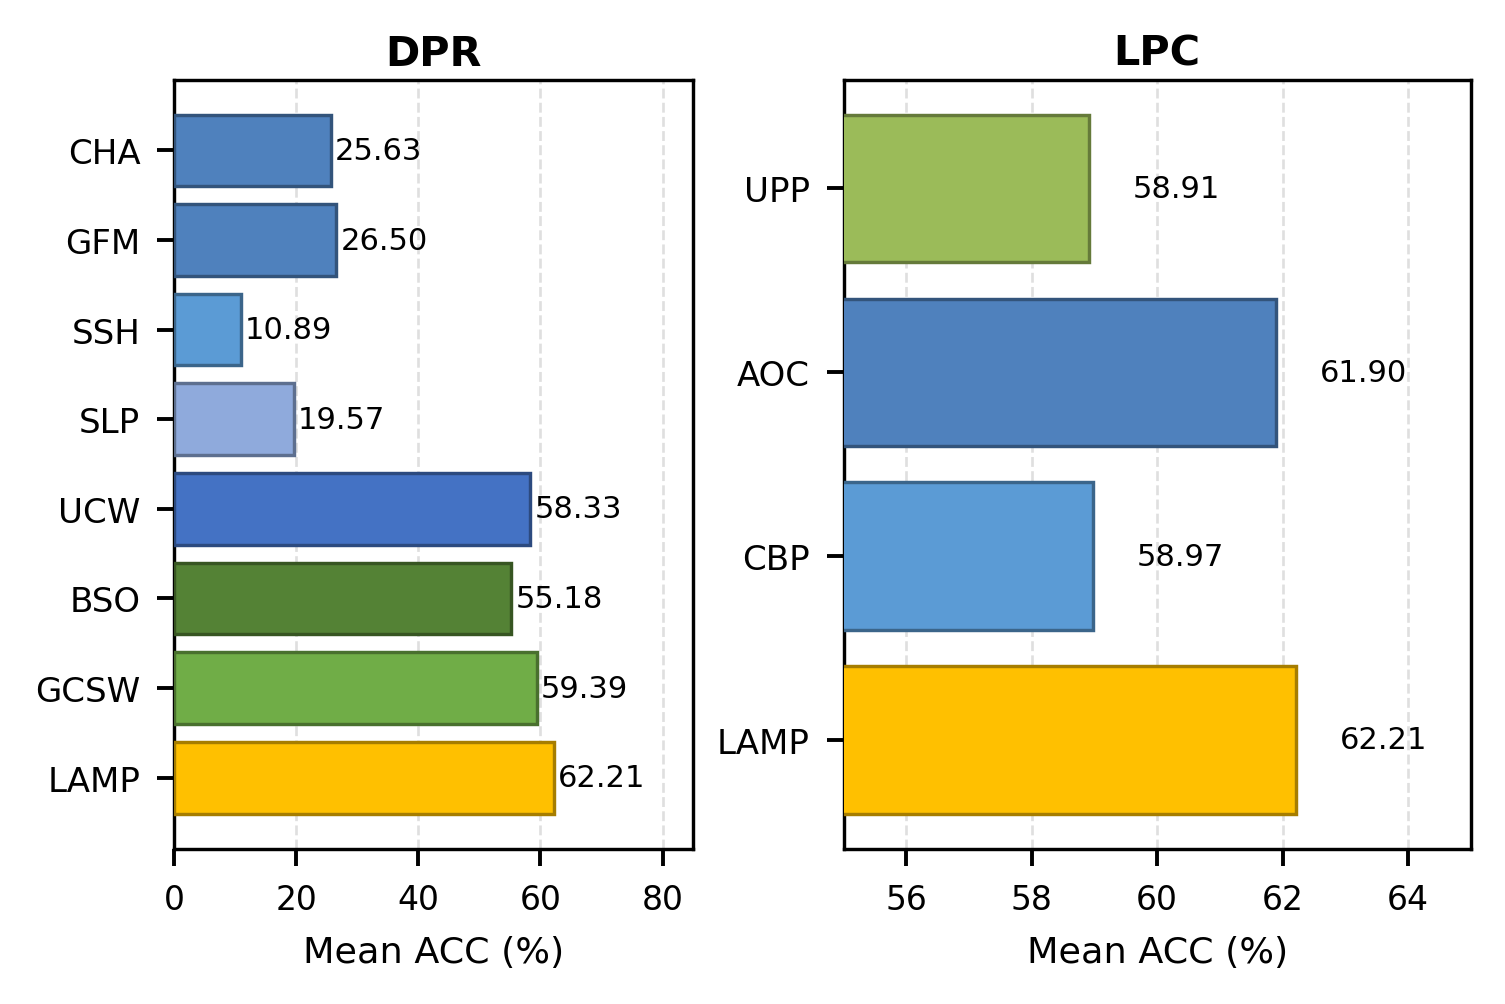
\includegraphics[width=0.88\linewidth]{figures/02_internal_module_ablations.png}
    \caption{Internal ablation of both Module}
    \label{fig:internal_module_ablations}
\end{figure}

We further replace the prior term inside long-tail prevalence calibration. Table ~\ref{tab:prevalence-internal-ablation} shows that removing prevalence calibration or replacing the real prior with a uniform prior reduces mean ACC, confirming that long-tailed prevalence is part of the full method.

\begin{figure*}[!t]
\centering
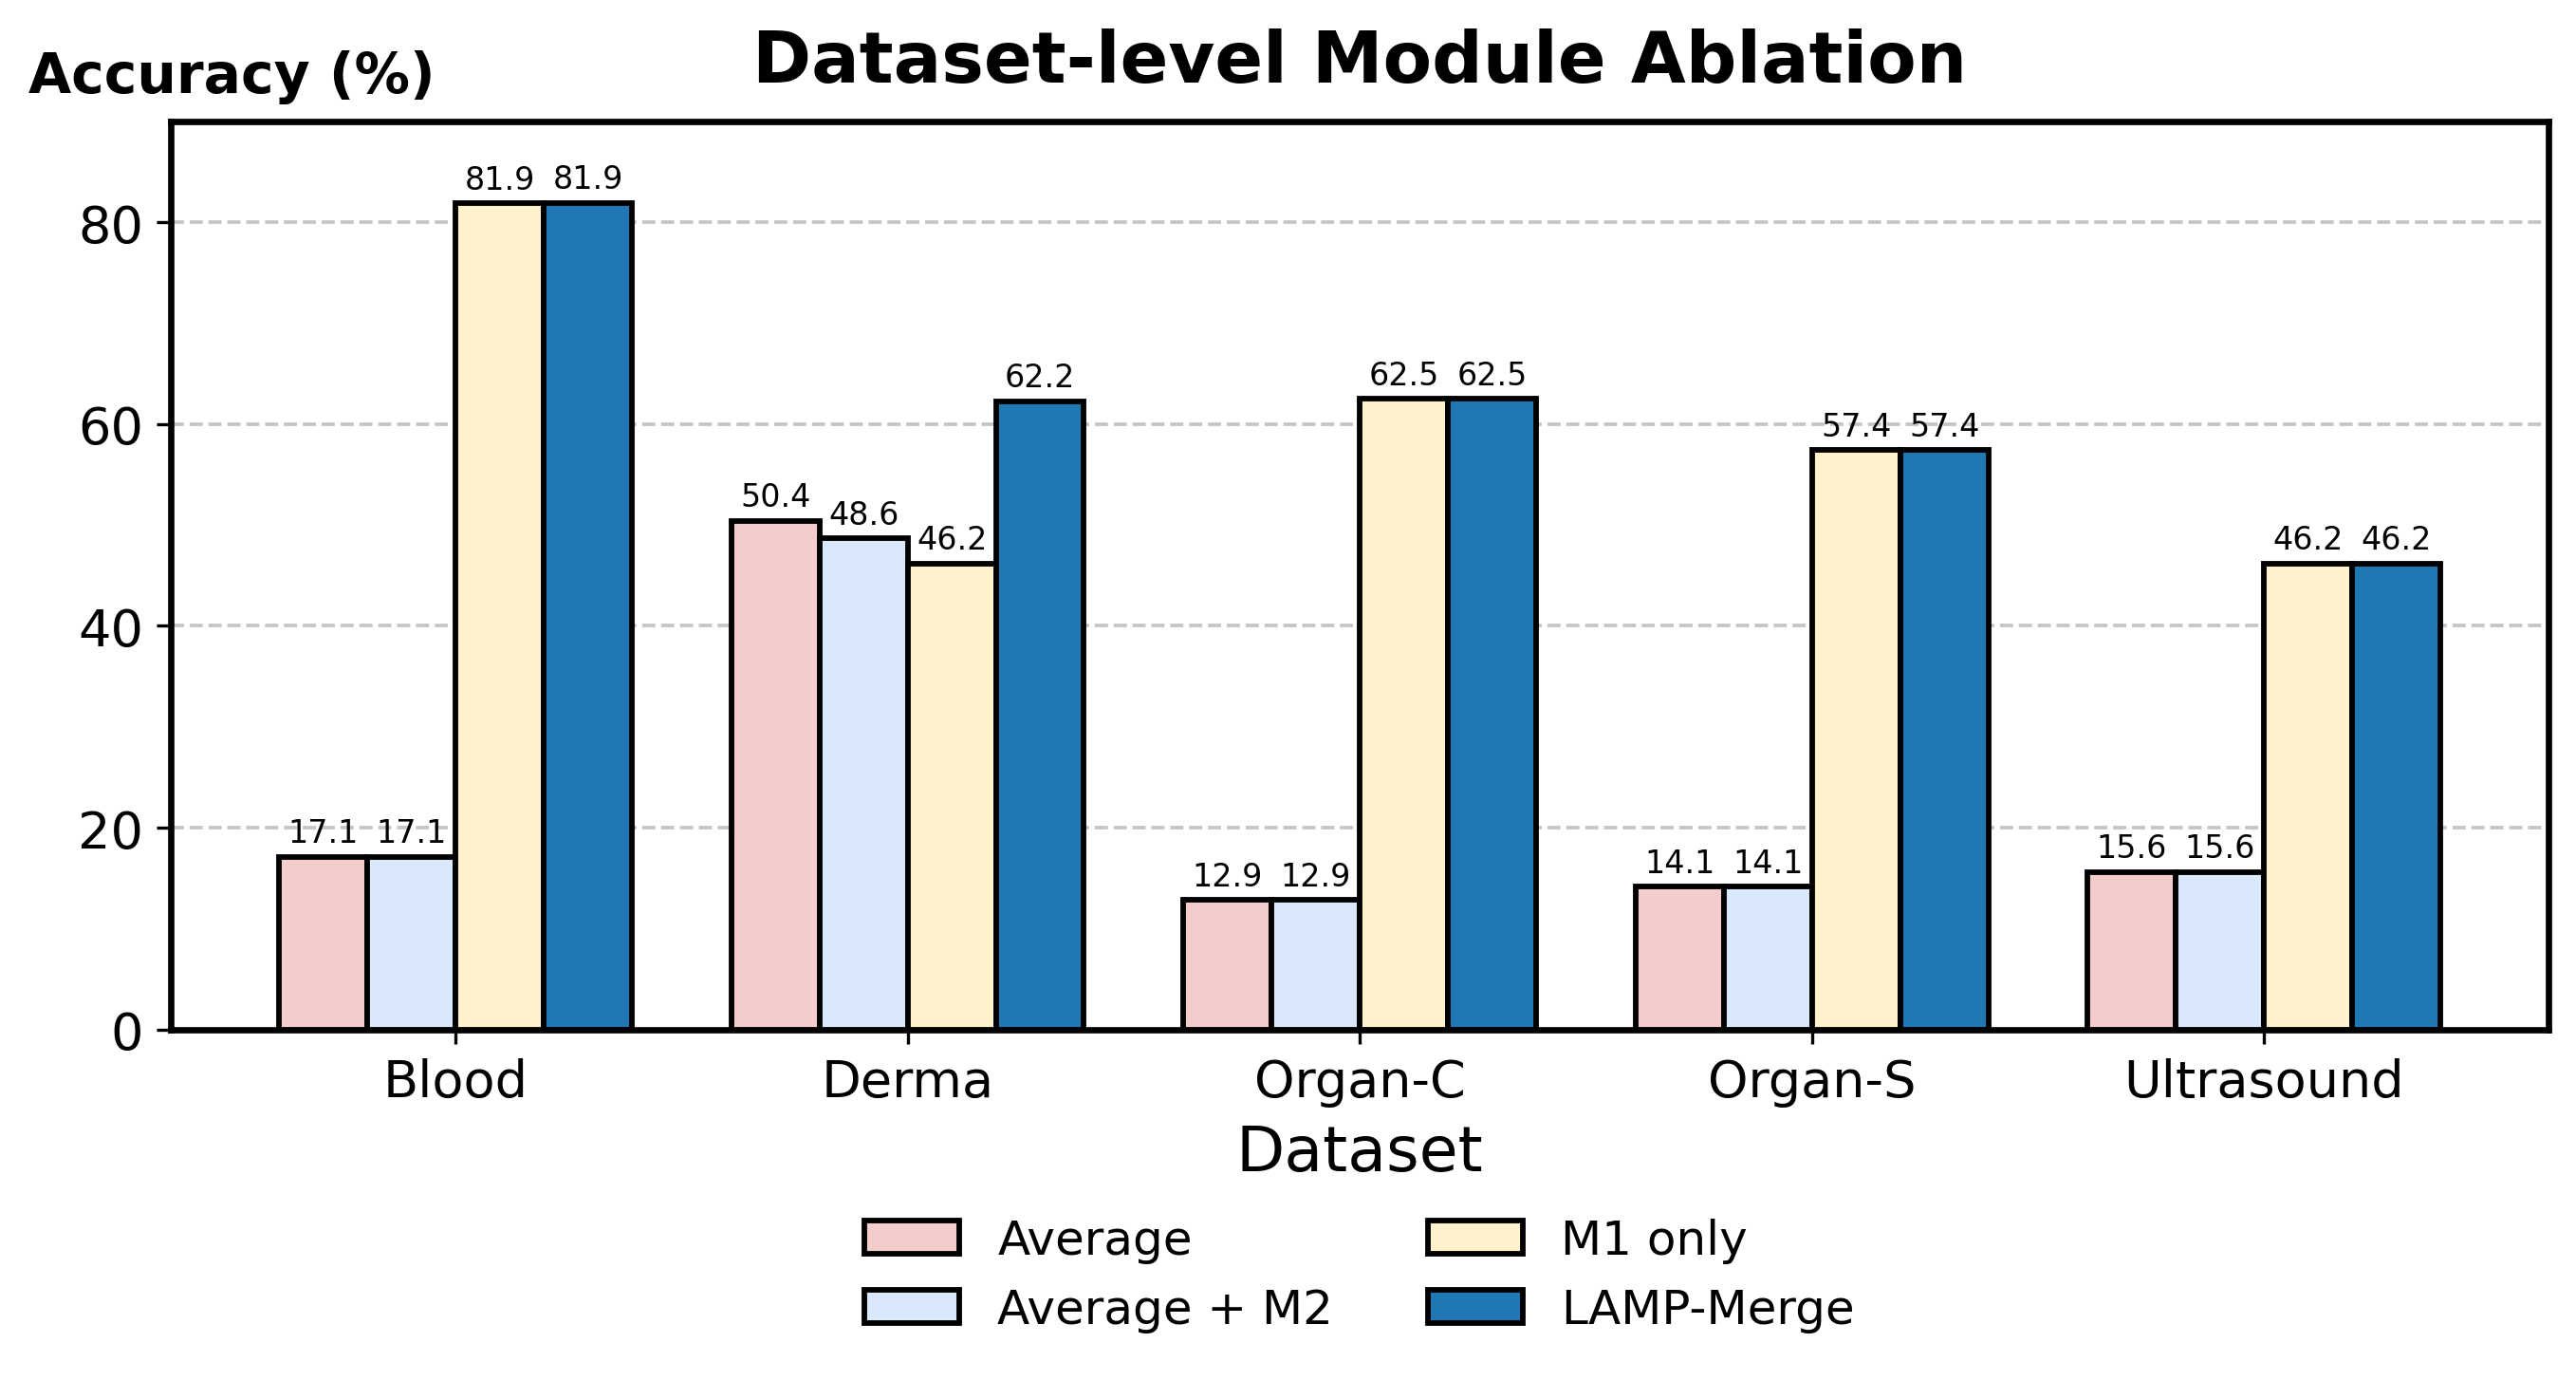
\includegraphics[width=0.92\textwidth]{figures/01_module_ablation_accuracy.png}
\caption{Dataset-level client-average accuracy in the module ablation. Each dataset contains 12 cells from four vision-model families and three client counts; each cell is averaged over three Dirichlet skew levels.}
\label{fig:dataset-ablation-acc}
\end{figure*}

\subsection{New-metric Diagnostic Experiment}
Although the main experiments use ACC for direct comparison, long-tailed medical distributions can allow single-class or few-class predictors to achieve high ACC\cite{BUDA2018249,5597285}. We therefore report collapse ratio, effective predicted classes, and predicted--true total variation.

\begin{table}[t]
\centering
\caption{Prediction-collapse diagnostics averaged over five medical datasets and four backbones per dataset. Ratio metrics are reported in percentage scale.}
\label{tab:collapse-key}
\scriptsize
\setlength{\tabcolsep}{3.5pt}
\renewcommand{\arraystretch}{1.35}
\begin{tabular}{lcc}
\noalign{\hrule height 1.25pt}
\rowcolor[HTML]{F2F2F2}
\textbf{Metric} & \textbf{LAMP-Merge} & \textbf{Best reference} \\
\hline \hline
Collapse ratio $\downarrow$ & 31.22 & 79.02 \\
\rowcolor{gray!10}
Effective classes $\uparrow$ & 7.13 & 2.05 \\
Pred-true TV $\downarrow$ & 12.62 & 70.40 \\
\noalign{\hrule height 1.25pt}
\end{tabular}
\end{table}

Table \ref{tab:collapse-key} compares LAMP-Merge with the best-performing baseline for each metric. \textbf{LAMP-Merge consistently and substantially outperforms the existing methods}. 

\subsection{Visualization Experiment}

To visualize the prediction-distribution changes measured by the new diagnostic metrics, we compare the predicted class allocation induced by LAMP-Merge with that of the strongest generic merge. The generic merge concentrates predictions on one class, whereas LAMP-Merge recovers a broader class allocation aligned with the test distribution.

\begin{figure}[t]
\centering
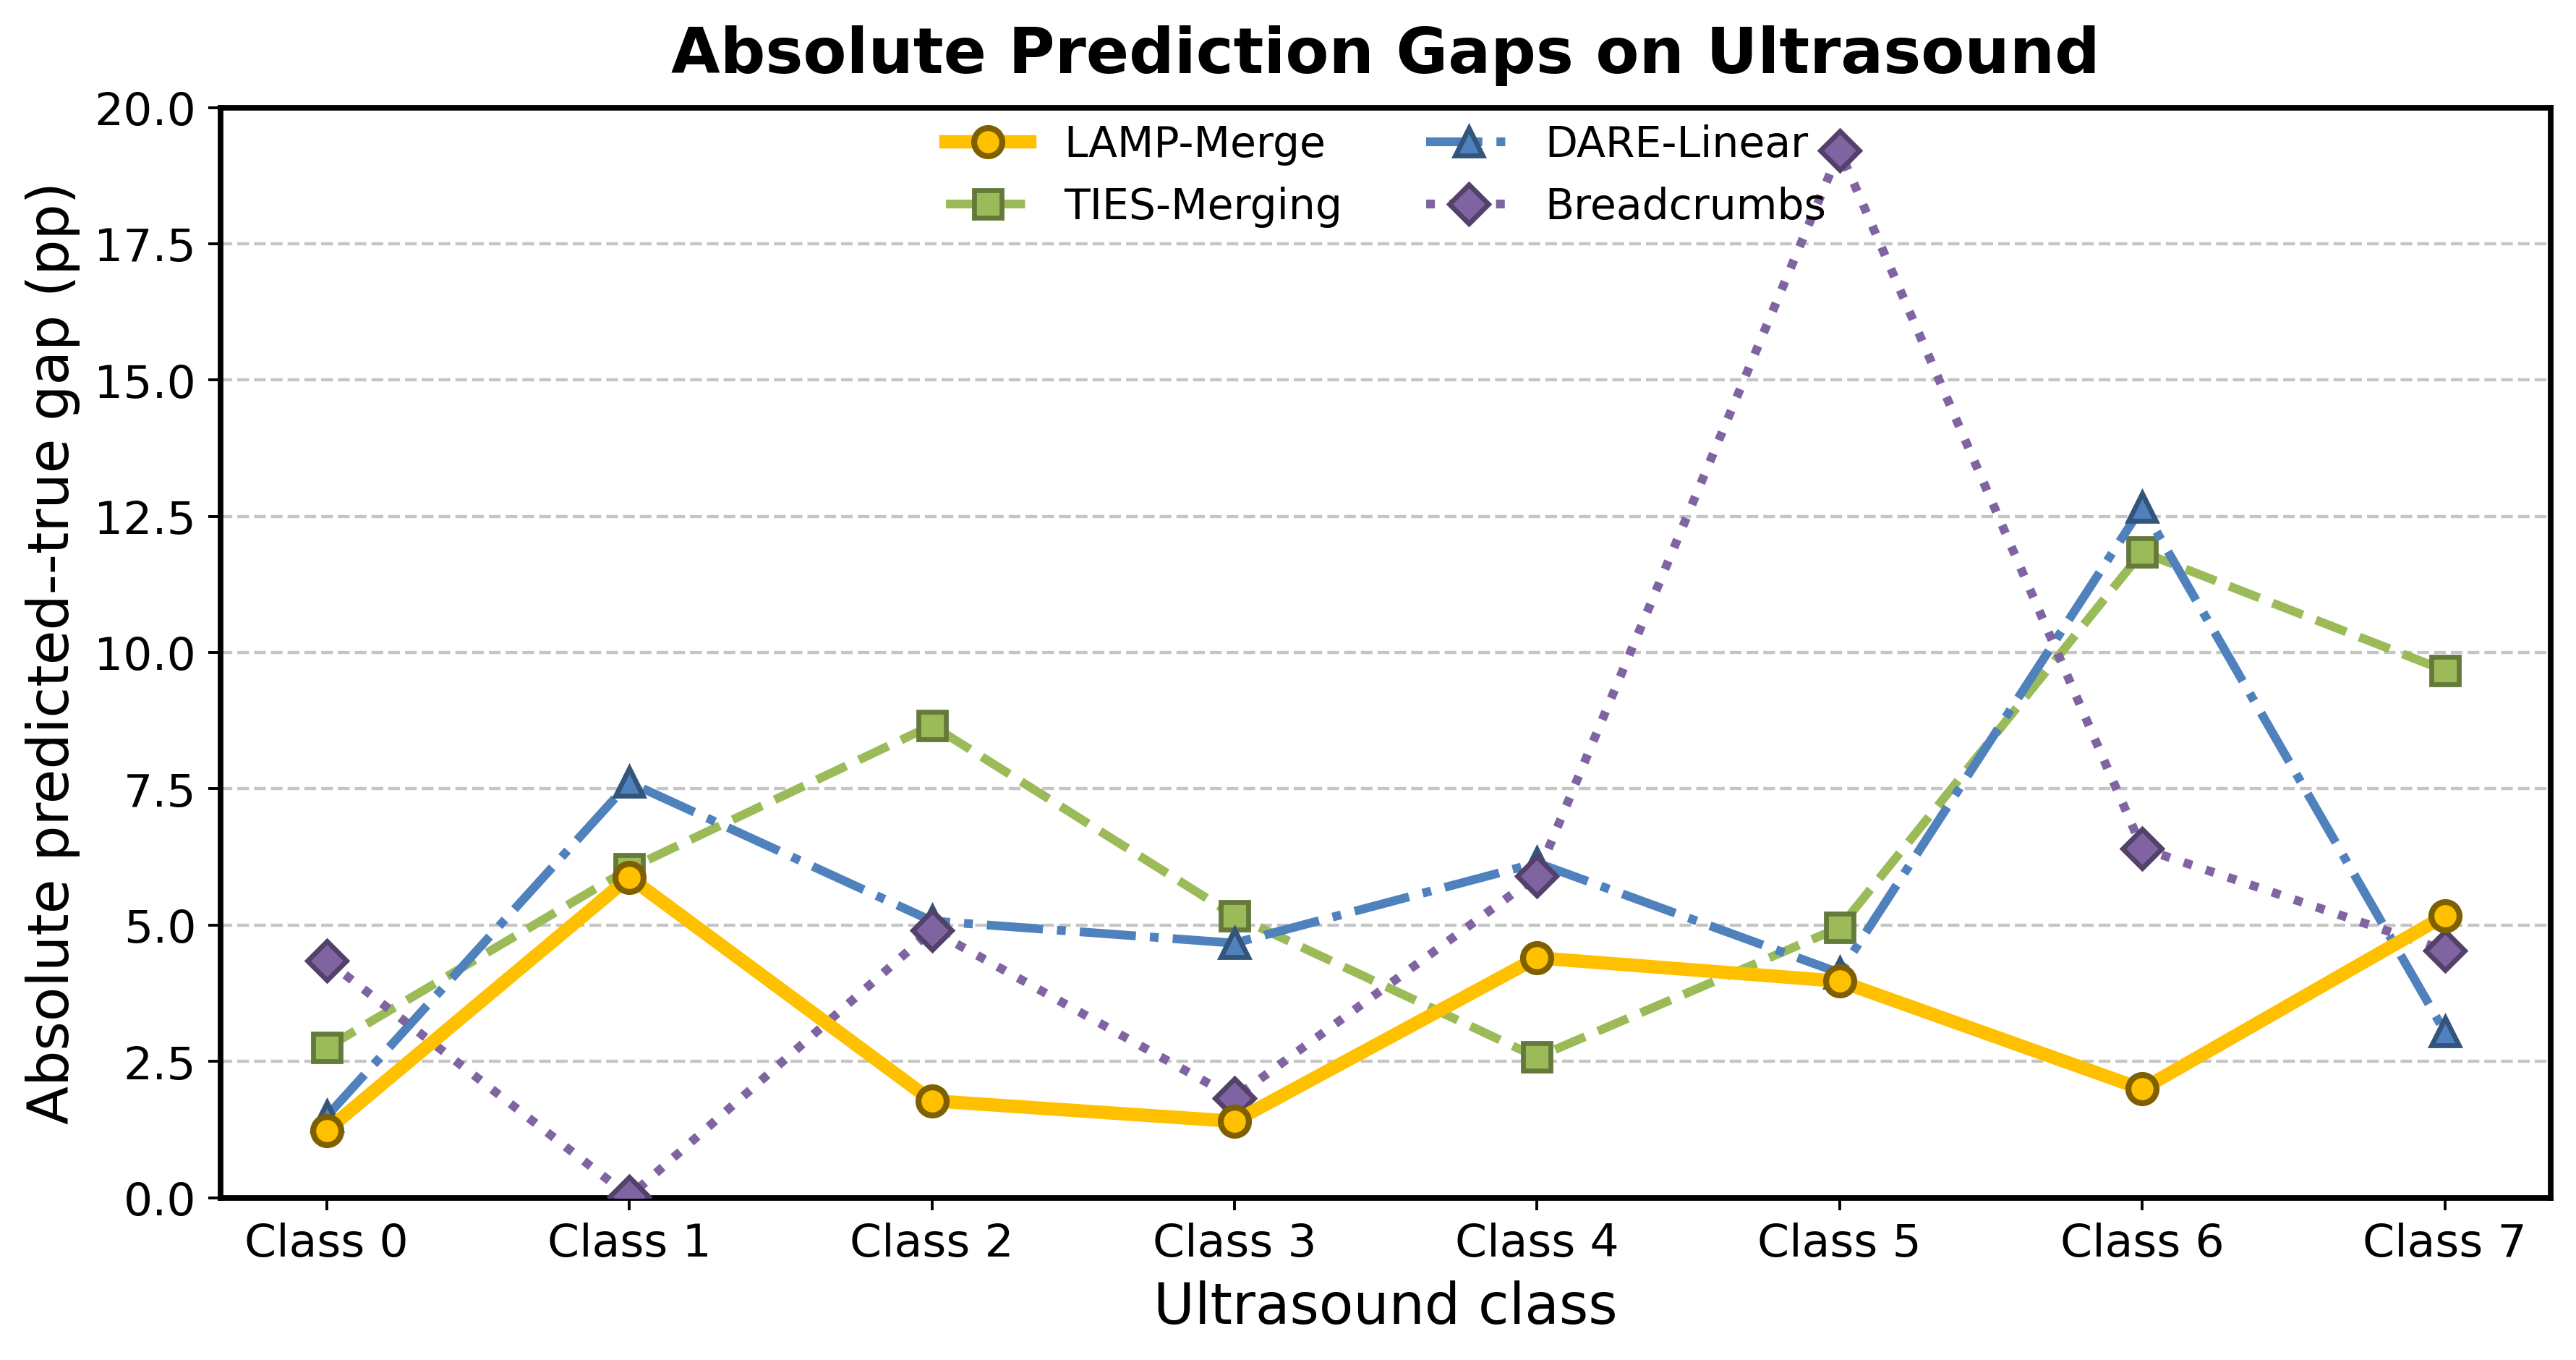
\includegraphics[width=\linewidth]{figures/04_ultrasound_class_distribution.png}
\caption{Predicted class distributions on Ultrasound, averaged over the four visual backbones, $K\in\{3,5,7\}$, and the three Dirichlet skew levels. The generic merge concentrates predictions on one class, while LAMP-Merge recovers a broader class allocation aligned with the test distribution.}
\label{fig:visual-chaosheng_predict}
\end{figure}

\subsection{Hyperparameter Analysis Experiment}
Fig.~\ref{fig:hparam-analysis-dpr} and Fig.~\ref{fig:hparam-analysis-lpc} evaluate the prototype-head scale $s$ and calibration strength $\lambda$ over 180 raw cells and 60 client-average cells. The default $s=20$ and $\lambda=5$ lie in broad stable regions, indicating that the gain is not produced by narrow hyperparameter tuning.

\begin{figure*}[t]
\centering

\includegraphics[width=0.92\textwidth]{figures/05_diagnostic_reconstruction_hparams.png}
\caption{Full-scope hyperparameter sensitivity for diagnostic prototype reconstruction.}
\label{fig:hparam-analysis-dpr}
\end{figure*}

\begin{figure*}[t]
\centering

\includegraphics[width=0.92\textwidth]{figures/06_prevalence_calibration_hparams.png}
\caption{Full-scope hyperparameter sensitivity for long-tail prevalence calibration.}
\label{fig:hparam-analysis-lpc}
\end{figure*}

\subsection{t-SNE Visualization Experiment}
Fig.~\ref{fig:tsne-analysis} uses t-SNE\cite{vanDerMaaten2008} only for analysis on Blood with ResNet, $K=3$, and $\beta=0.01$. LAMP-Merge retains separated output-probability groups, while generic merges exhibit compressed or entangled predictive representations.

\begin{figure*}[t]
\centering
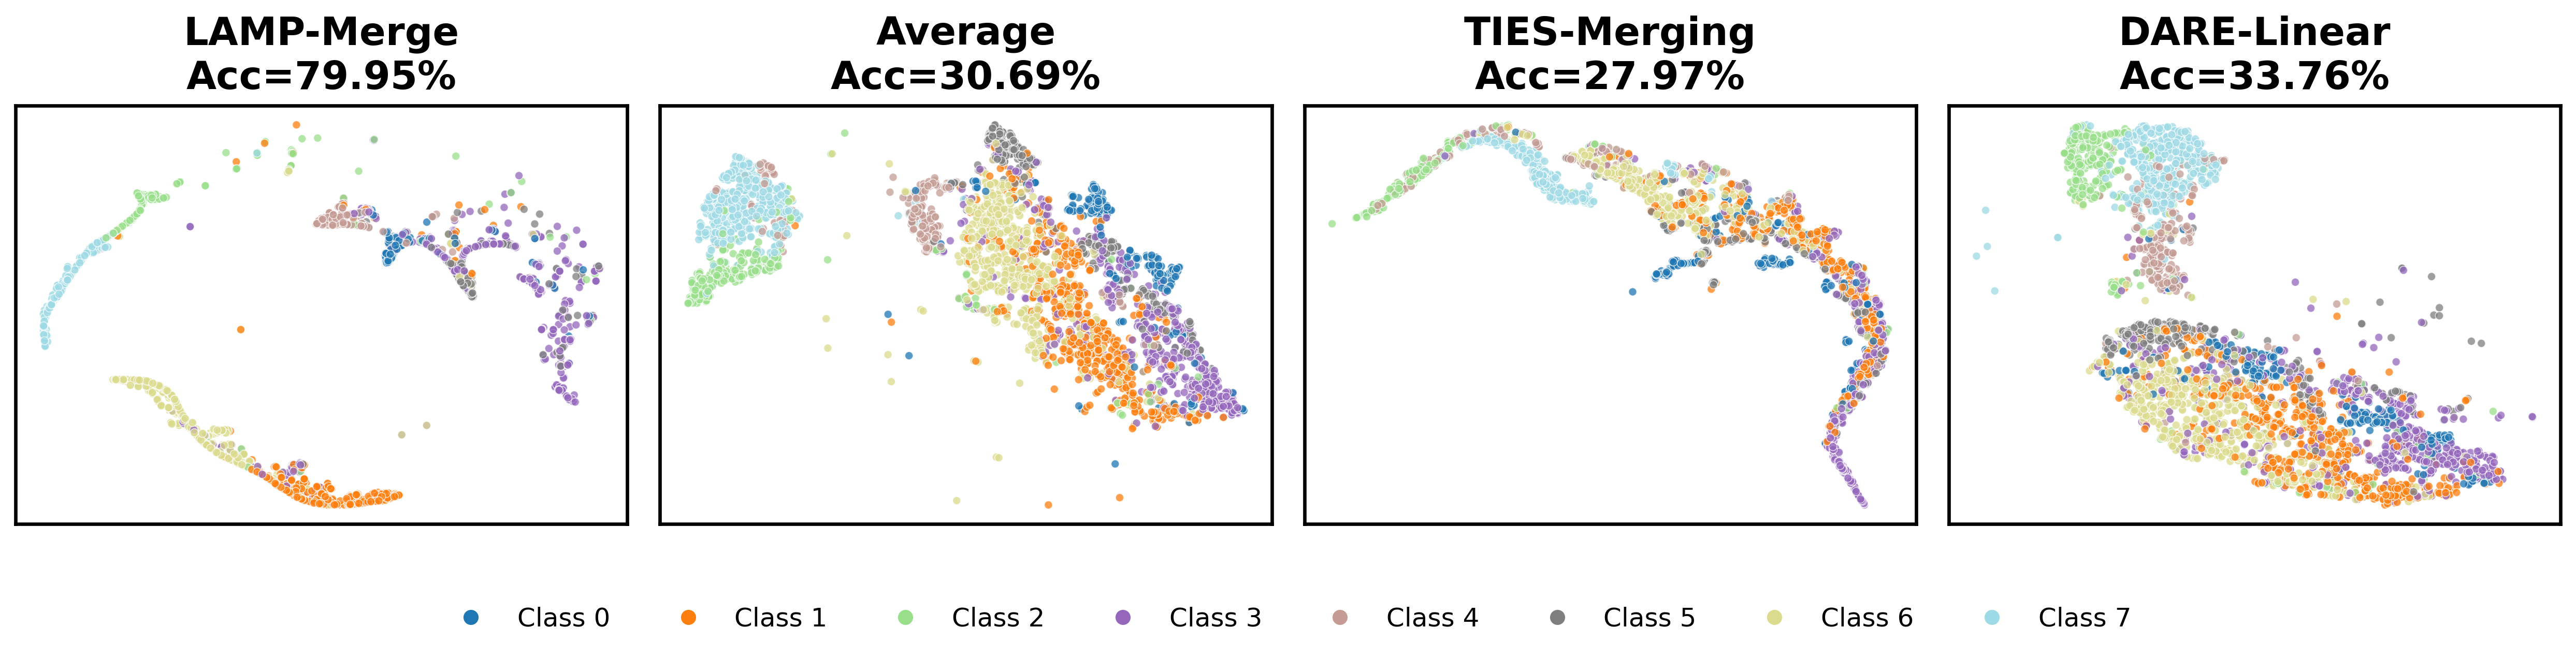
\includegraphics[width=0.98\textwidth]{figures/07_tsne_output_probability.png}
\caption{Joint t-SNE of test-image output-probability representations on Blood; from left to right, LAMP-Merge, weight averaging, TIES-Merging, and DARE-Linear.}
\label{fig:tsne-analysis}
\end{figure*}


\section{Conclusion}

We studied \textbf{one-shot asynchronous medical model merging}, where independently trained hospital models must be fused without federated optimization rounds and without exposing raw medical images to the server. Our empirical analysis shows that generic model-merging methods suffer from \textbf{aggregation-induced predictive collapse} under incomplete local diagnostic coverage. We further show that, on long-tailed medical datasets, such collapse can be masked by raw accuracy. We therefore introduce the Long-tail Prevalence Calibration module and perform secondary evaluation using macro recall, macro-F1, and predictive-distribution diagnostics\cite{BUDA2018249,5597285}.

Taken together, the full-scope comparisons, module ablations, and prediction-distribution diagnostics establish a consistent mechanism: class-level support-weighted evidence reconstructs discriminative directions for locally absent diagnoses, while bounded prevalence calibration retains clinically meaningful imbalance without reintroducing majority-class collapse.

LAMP-Merge addresses these two properties through a concise two-module design. Future work will extend its applicability in two directions: first, from medical image classification to segmentation, detection, and multimodal diagnostic tasks; and second, toward stronger privacy-preserving mechanisms, such as differential privacy and secure aggregation, to further reduce potential privacy risks associated with class-level statistics\cite{kaissis2020secure,geyer2017differentially,abadi2016deep}. We will also explore deployment and validation in larger-scale real-world multicenter healthcare settings.

\bibliography{aaai2026}
\appendix
\section{Supplementary Results and Analysis}

\subsection{Evaluation Datasets}

% \subsubsection{Evaluation Datasets}
The five MedMNIST v2 benchmarks\cite{yang2023medmnist} cover blood-cell microscopy, dermoscopy, abdominal CT organ slices, and ultrasound images. They involve cell morphology recognition, skin-lesion diagnosis, organ-structure recognition, and ultrasound-structure discrimination:
\begin{itemize}
\item \textbf{Blood}: an eight-class blood-cell microscopy dataset for hematological morphology classification, focusing on fine-grained cellular appearance and inter-class morphological similarity.
\item \textbf{Derma}: a seven-class dermoscopic skin-lesion dataset, characterized by strong long-tailed prevalence and visually subtle lesion categories.
\item \textbf{Organ-C}: an 11-class abdominal CT dataset in the coronal view, evaluating organ-category recognition under grayscale cross-sectional imaging.
\item \textbf{Organ-S}: an 11-class abdominal CT dataset in the sagittal view, complementing Organ-C with a different anatomical imaging plane.
\item \textbf{Ultrasound}: an eight-class ultrasound image dataset, covering structure recognition under modality-specific speckle noise and low-contrast boundaries.
\end{itemize}
Together, these benchmarks provide a systematic testbed for evaluating cross-modality robustness, class-discriminative capability, and task generalization under different medical image types and class-distribution conditions.

\begin{table*}[t]
\centering
\caption{Dataset statistics and class-level sample placeholders for the five medical image benchmarks. The sample column is reserved for representative images.}
\label{tab:dataset-statistics}
\scriptsize
\renewcommand{\arraystretch}{1.32}
\setlength{\tabcolsep}{8pt}
\begin{tabular}{l||lcc:c:c}
\noalign{\hrule height 1.25pt}
\rowcolor[HTML]{F2F2F2}
\textbf{Dataset} & \textbf{Class} & \textbf{Train} & \textbf{Test} & \textbf{Total} & \textbf{Sample} \\
\hline \hline
\multirow{5}{*}{Blood} & Class 1 & - & - & - & * \\
& Class 2 & - & - & - & * \\
& $\cdots$ & - & - & - & * \\
& Class 8 & - & - & - & * \\
\cline{2-6}
& \textbf{Total} & \textbf{-} & \textbf{-} & \textbf{-} & - \\
\hline \hline
\multirow{5}{*}{Derma} & Class 1 & - & - & - & * \\
& Class 2 & - & - & - & * \\
& $\cdots$ & - & - & - & * \\
& Class 7 & - & - & - & * \\
\cline{2-6}
& \textbf{Total} & \textbf{-} & \textbf{-} & \textbf{-} & - \\
\hline \hline
\multirow{5}{*}{Organ-C} & Class 1 & - & - & - & * \\
& Class 2 & - & - & - & * \\
& $\cdots$ & - & - & - & * \\
& Class 11 & - & - & - & * \\
\cline{2-6}
& \textbf{Total} & \textbf{-} & \textbf{-} & \textbf{-} & - \\
\hline \hline
\multirow{5}{*}{Organ-S} & Class 1 & - & - & - & * \\
& Class 2 & - & - & - & * \\
& $\cdots$ & - & - & - & * \\
& Class 11 & - & - & - & * \\
\cline{2-6}
& \textbf{Total} & \textbf{-} & \textbf{-} & \textbf{-} & - \\
\hline \hline
\multirow{5}{*}{Ultrasound} & Class 1 & - & - & - & * \\
& Class 2 & - & - & - & * \\
& $\cdots$ & - & - & - & * \\
& Class 8 & - & - & - & * \\
\cline{2-6}
& \textbf{Total} & \textbf{-} & \textbf{-} & \textbf{-} & - \\
\noalign{\hrule height 1.25pt}
\end{tabular}
\end{table*}

\begin{figure*}[t]
\centering

\includegraphics[width=0.86\textwidth,height=0.58\textheight,keepaspectratio]{figures/dataset_examples.png}
\caption{Representative training images from the five medical image datasets used in the experiments. The class IDs are shown only to illustrate category diversity within each dataset.}
\label{fig:dataset-examples}
\end{figure*}

\subsection{Detailed Ablation Configurations}
\label{app:ablation-configurations}

All diagnostic-prototype substitutions retain long-tail prevalence calibration and vary only prototype semantics or support-count weighting:
\begin{itemize}
\setlength{\itemsep}{0pt}
\item \textbf{LAMP-Merge} uses \(p_c=\sum_i\alpha_{i,c}\mu_{i,c}\), where \(e_{i,c}=(n_{i,c}+1)^\gamma\mathbf{1}[n_{i,c}>0]\) determines the class-support reliability.
\item \textbf{Classifier-head aggregation} replaces the reference-space class prototype by the local classifier-head direction, i.e., \(\mu_{i,c}\leftarrow h_{i,c}\).
\item \textbf{Global-feature mean} removes class conditioning by setting \(\mu_{i,c}\leftarrow g\) for all \(c\), where \(g\) is the class-agnostic global reference-feature mean.
\item \textbf{Support-only synthetic head} removes image evidence by replacing each prototype with a fixed random unit direction \(u_c\), i.e., \(p_c\leftarrow u_c\), \(\|u_c\|_2=1\).
\item \textbf{Shuffled-label prototype} preserves prototype magnitudes but permutes diagnostic semantics, i.e., \(p_c\leftarrow p_{\sigma(c)}\), where \(\sigma\) is a random permutation over diagnosis labels.
\item \textbf{Uniform client weight} replaces support-weighted aggregation with equal weights among clients containing class \(c\), i.e., \(\alpha_{i,c}\leftarrow \mathbf{1}[n_{i,c}>0]/\sum_j\mathbf{1}[n_{j,c}>0]\).
\item \textbf{Binary support only} replaces fine-grained support and prevalence counts with class-presence indicators, i.e., \(n_{i,c},m_{i,c}\leftarrow \mathbf{1}[n_{i,c}>0]\).
\item \textbf{Global client-size weight} uses the total client support \(N_i=\sum_k n_{i,k}\) rather than class-specific support, i.e., \(e_{i,c}\leftarrow (N_i+1)^\gamma\mathbf{1}[n_{i,c}>0]\).
\end{itemize}

The long-tail prevalence substitutions vary only the class prior used by the calibration bias:
\begin{itemize}
\setlength{\itemsep}{0pt}
\item \textbf{LAMP-Merge} estimates the empirical class prior as \(\pi_c=\sum_i m_{i,c}/\sum_k\sum_i m_{i,k}\).
\item \textbf{No prevalence calibration} removes the calibration bias by setting \(b_c\leftarrow0\).
\item \textbf{Uniform prevalence prior} removes long-tail prevalence by setting \(\pi_c\leftarrow 1/C\), where \(C\) is the number of diagnosis classes.
\end{itemize}

\subsubsection{2) Additional Theoretical Analysis}
Let $\mu_c^\star$ denote the true class mean in the shared reference space. If client class features have bounded second moments, the prototype estimation error satisfies
\begin{equation}
\mathrm{E}\|p_c-\mu_c^\star\|_2^2
\le
\sum_i \alpha_{i,c}^2\frac{\sigma_c^2}{n_{i,c}}
+ \mathrm{Bias}_c^2.
\end{equation}
This upper bound shows that support counts directly control the variance of class-prototype estimation. A client that does not observe class $c$ should not contribute evidence for that class, and a client with more samples should contribute more, but only sublinearly.

Let the true margin between classes $c$ and $d$ for sample $x$ be
\begin{equation}
\Delta_{c,d}(x)=(\mu_c^\star)^\top z-(\mu_d^\star)^\top z.
\end{equation}
When the prototype error satisfies
\begin{equation}
\|p_c-\mu_c^\star\|_2+\|p_d-\mu_d^\star\|_2
<
\frac{\Delta_{c,d}(x)}{\|z\|_2},
\end{equation}
the estimated prototypes preserve the class order between $c$ and $d$.

The role of long-tail prevalence calibration is to introduce long-tail priors in a bounded manner. For prevalence counts $m_{i,c}$, the class prior is
\begin{equation}
\pi_c=\frac{\sum_i m_{i,c}}{\sum_k \sum_i m_{i,k}},
\end{equation}
and the centered log-prior bias is
\begin{equation}
b_c=\lambda\left(\log\pi_c-\frac{1}{C}\sum_k\log\pi_k\right).
\end{equation}
As long as $\lambda$ is bounded, long-tail prevalence calibration does not replace the discriminative directions reconstructed by diagnostic prototype reconstruction; it only calibrates the output toward the real class prevalence. This explains why using long-tail prevalence calibration alone is insufficient, while full LAMP-Merge remains both non-collapsed and prevalence-aware.

\subsection{Metric Definitions}
\label{app:metric-geometry}

Let \(y_n\) and \(\hat{y}_n\) denote the true and predicted labels of the \(n\)-th test sample. Let \(q_c=N^{-1}\sum_n\mathbf{1}[\hat{y}_n=c]\) be the predicted-class distribution, \(p_c=N^{-1}\sum_n\mathbf{1}[y_n=c]\) the true class distribution, and \(\mathcal{C}_{\mathrm{test}}=\{c\mid \sum_n\mathbf{1}[y_n=c]>0\}\) the set of classes observed in the test set. We use:
\begin{itemize}
\setlength{\itemsep}{0pt}
\item \(\mathrm{BA}=|\mathcal{C}_{\mathrm{test}}|^{-1}\sum_{c\in\mathcal{C}_{\mathrm{test}}}\mathrm{Recall}_c\), balanced accuracy or macro recall, which measures whether all observed diagnosis classes are recalled.
\item \(\mathrm{MacroF1}=|\mathcal{C}_{\mathrm{test}}|^{-1}\sum_{c\in\mathcal{C}_{\mathrm{test}}}\mathrm{F1}_c\), class-balanced precision-recall quality that penalizes majority-only predictions.
\item \(\rho=\max_c q_c\), the prediction-collapse ratio, which measures concentration on a single diagnosis class.
\item \(C_{\mathrm{eff}}=\exp\left(-\sum_c q_c\log q_c\right)\), the effective number of predicted classes.
\item \(\mathrm{TV}(q,p)=\frac{1}{2}\sum_c |q_c-p_c|\), the total variation distance between predicted and true class distributions.
\end{itemize}

\end{document}
